\documentclass[12pt]{article}

\usepackage[margin=1in]{geometry}
\usepackage{graphicx}

\usepackage{amsmath}
\usepackage{caption}
\usepackage{subcaption}
\usepackage{hyperref}
\usepackage{listings}
\usepackage{color}

\definecolor{dkgreen}{rgb}{0,0.6,0}
\definecolor{gray}{rgb}{0.5,0.5,0.5}
\definecolor{mauve}{rgb}{0.58,0,0.82}

\lstset{frame=tb,
  language=C++,
  aboveskip=3mm,
  belowskip=3mm,
  showstringspaces=false,
  columns=flexible,
  basicstyle={\small\ttfamily},
  numbers=none,
  numberstyle=\tiny\color{gray},
  keywordstyle=\color{blue},
  commentstyle=\color{dkgreen},
  stringstyle=\color{mauve},
  breaklines=true,
  breakatwhitespace=true,
  tabsize=3
}

\usepackage[T1]{fontenc}
\usepackage{sectsty}
\sectionfont{\bfseries\Large\raggedright}

\newcommand\T{\rule{0pt}{2.6ex}} % insert \T to add upwards vertical space
\newcommand\B{\rule[-1.2ex]{0pt}{0pt}} % insert \B to add downwards vertical space

\setlength{\parindent}{0in}
\pagestyle{empty}


\begin{document}

\thispagestyle{empty}

{\scshape Émile Greer (100914184) and Alex Vena ()} \hfill {Project V1 \scshape \large} \hfill {\scshape COMP 3005 - Winter 2024}
 
\smallskip
\hrule
\bigskip

\section*{Conceptual Design}
\subsection*{Entity-Relation Diagram}

\subsection*{Assumptions}
\begin{enumerate}
    \item If an attribute is the same for every row in a table, we ommit that attribute. Examples include the 'duration' attribute in the event tables. In many cases, 'duration' is always 0.0 - for those tables we ommit the 'duration' attribute entirely.
    \item The 'related\_events' attribute cannot refer to an event from a different match. This assumption was made for data validation and to reduce json\_loader execution times.
\end{enumerate}

\section*{Reduction to Relation Schemas}
You can access the full schema here: \href{https://dbdiagram.io/d/soccer_schema-66196f2f03593b6b61de1763}{Reduction to Relational Schemas}.

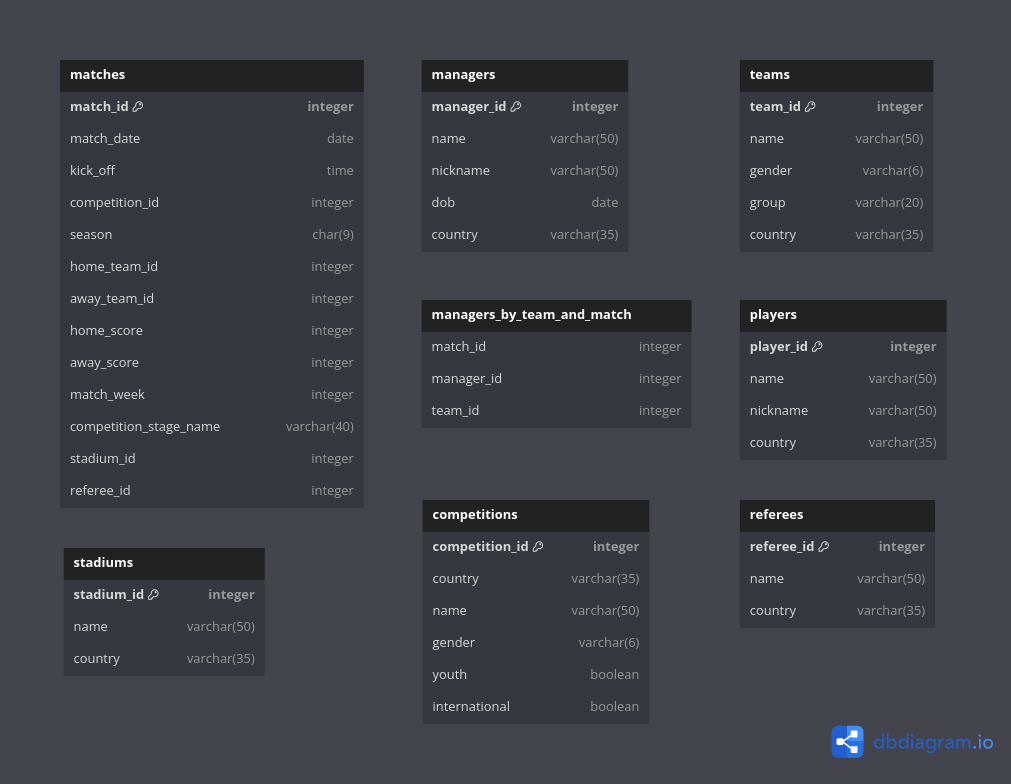
\includegraphics[width=\textwidth]{reduction/1.png}
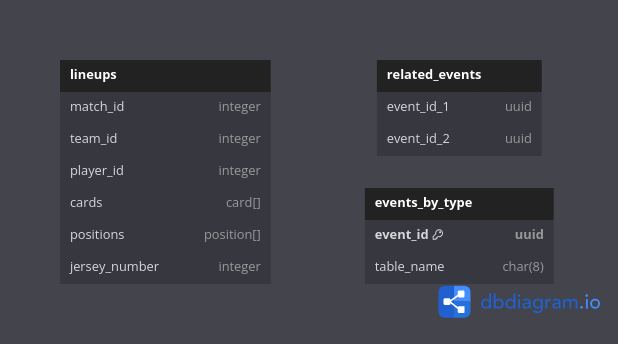
\includegraphics[width=\textwidth]{reduction/2.png}
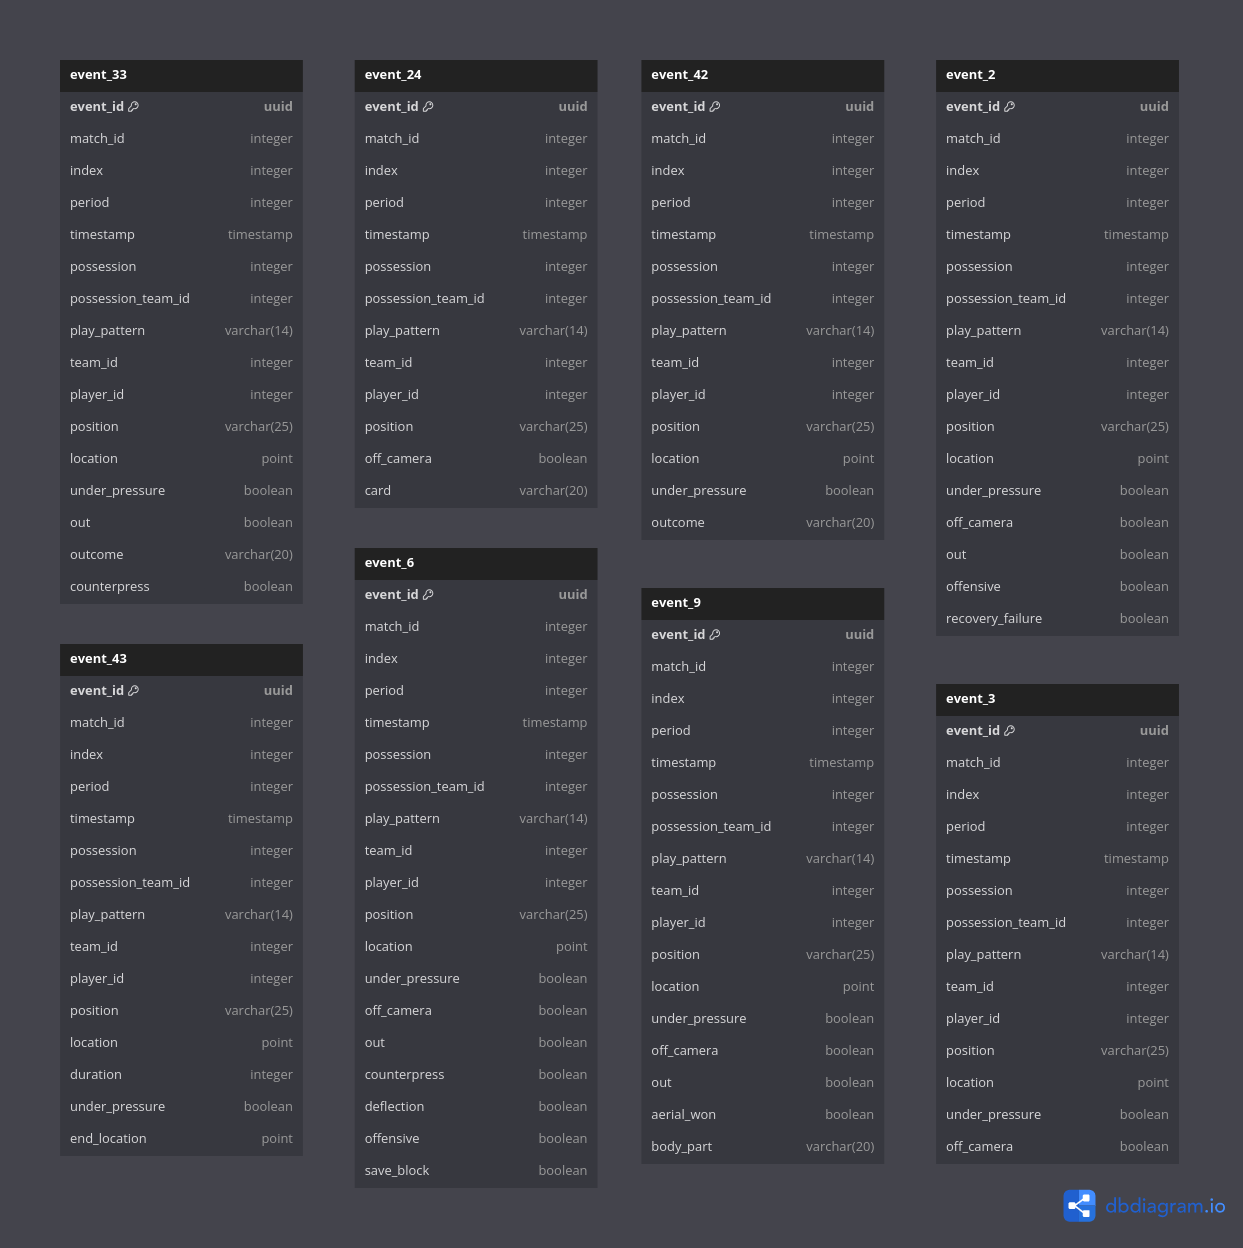
\includegraphics[width=\textwidth]{reduction/3.png}
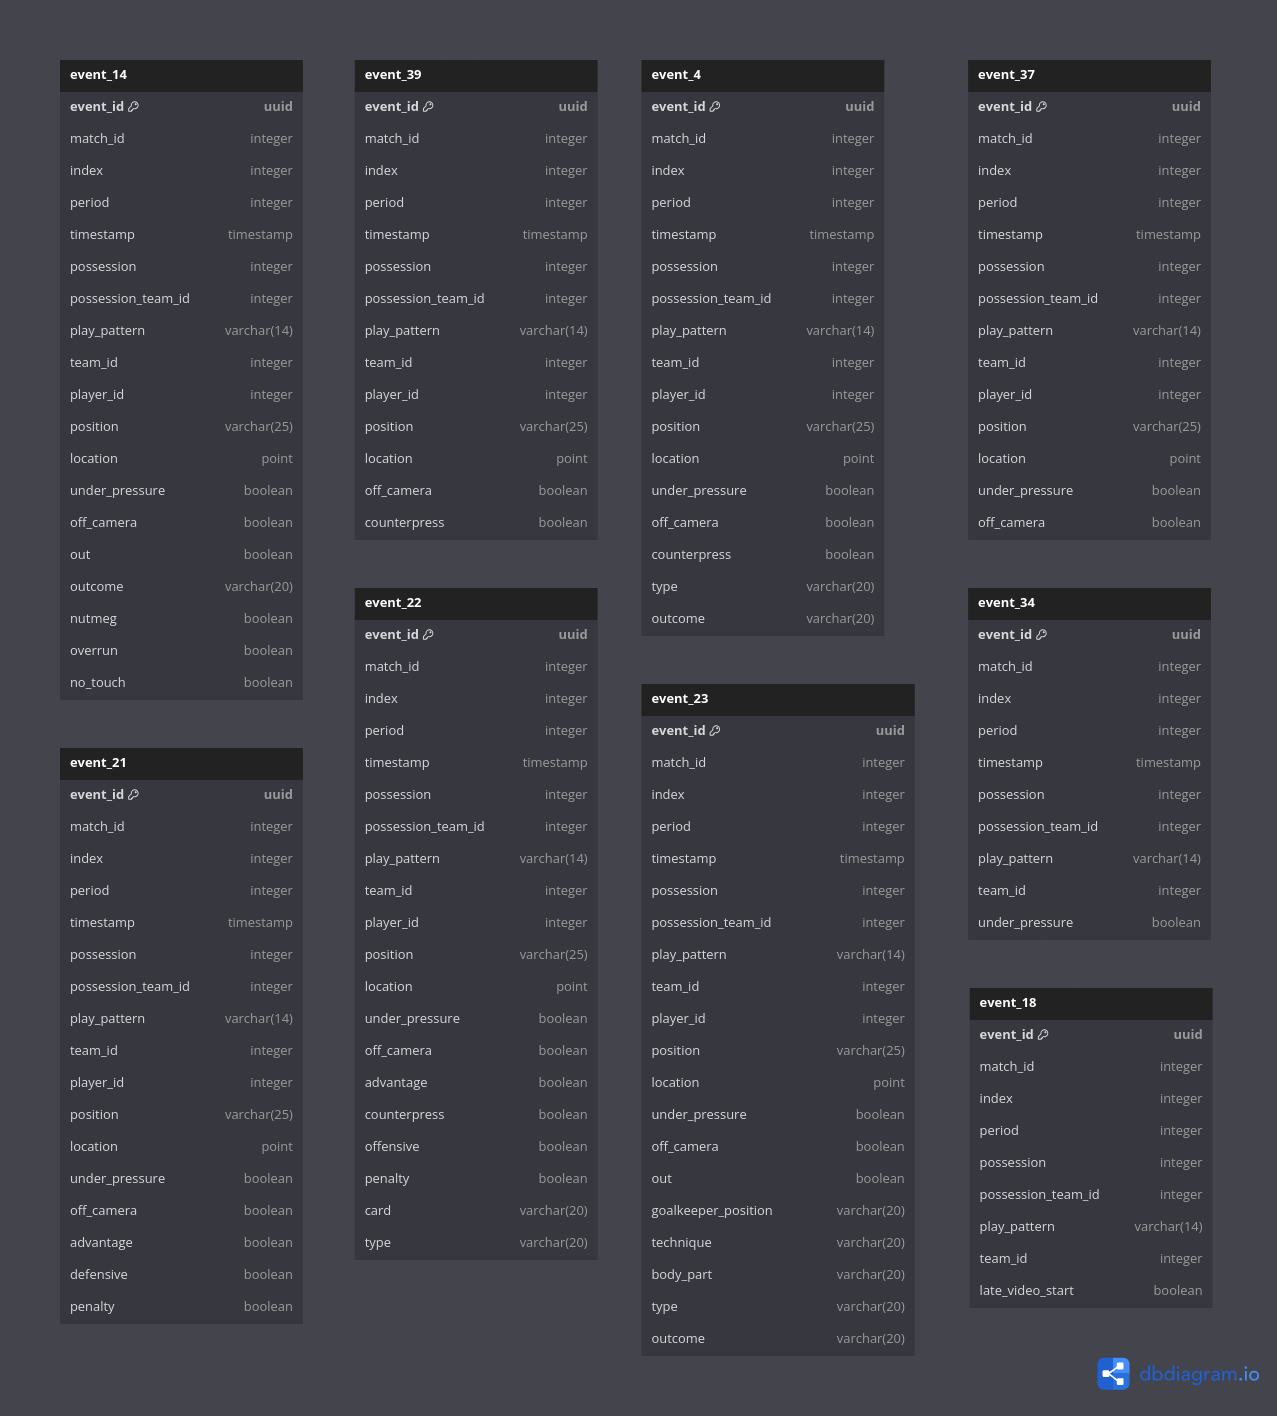
\includegraphics[width=\textwidth]{reduction/4.png}
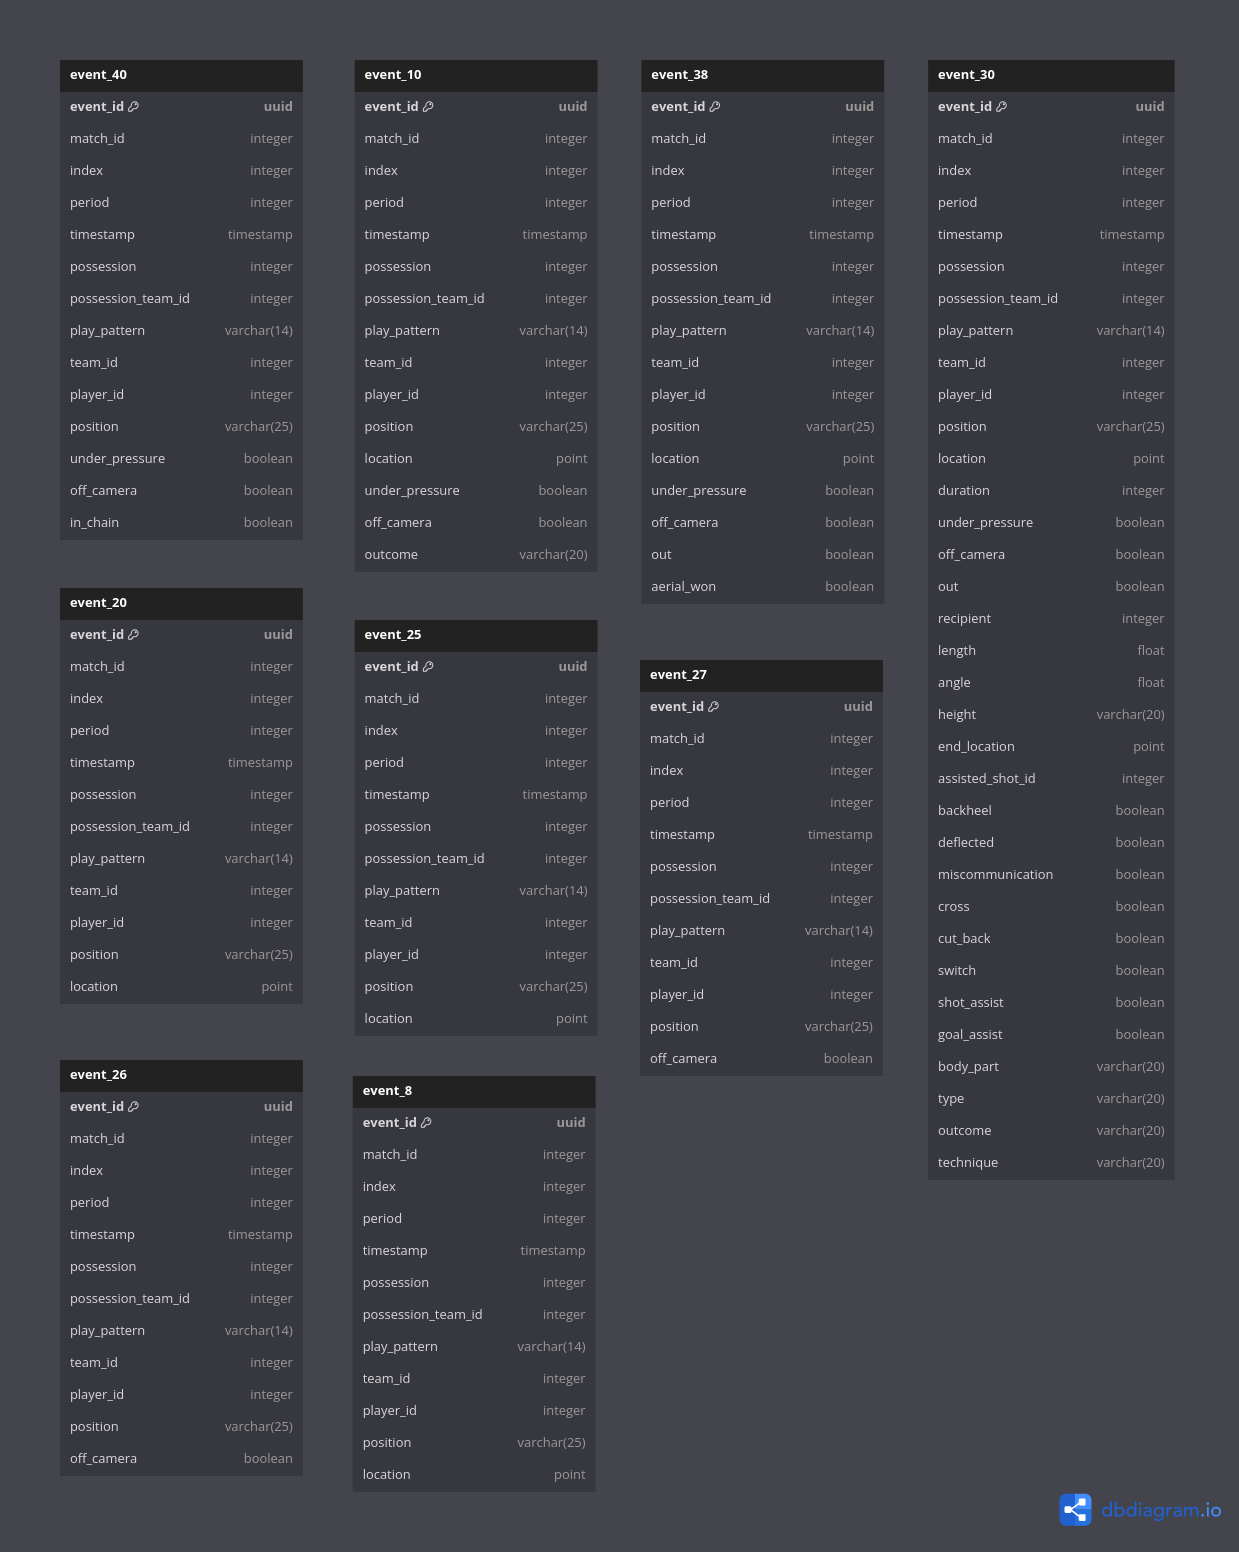
\includegraphics[width=\textwidth]{reduction/5.png}
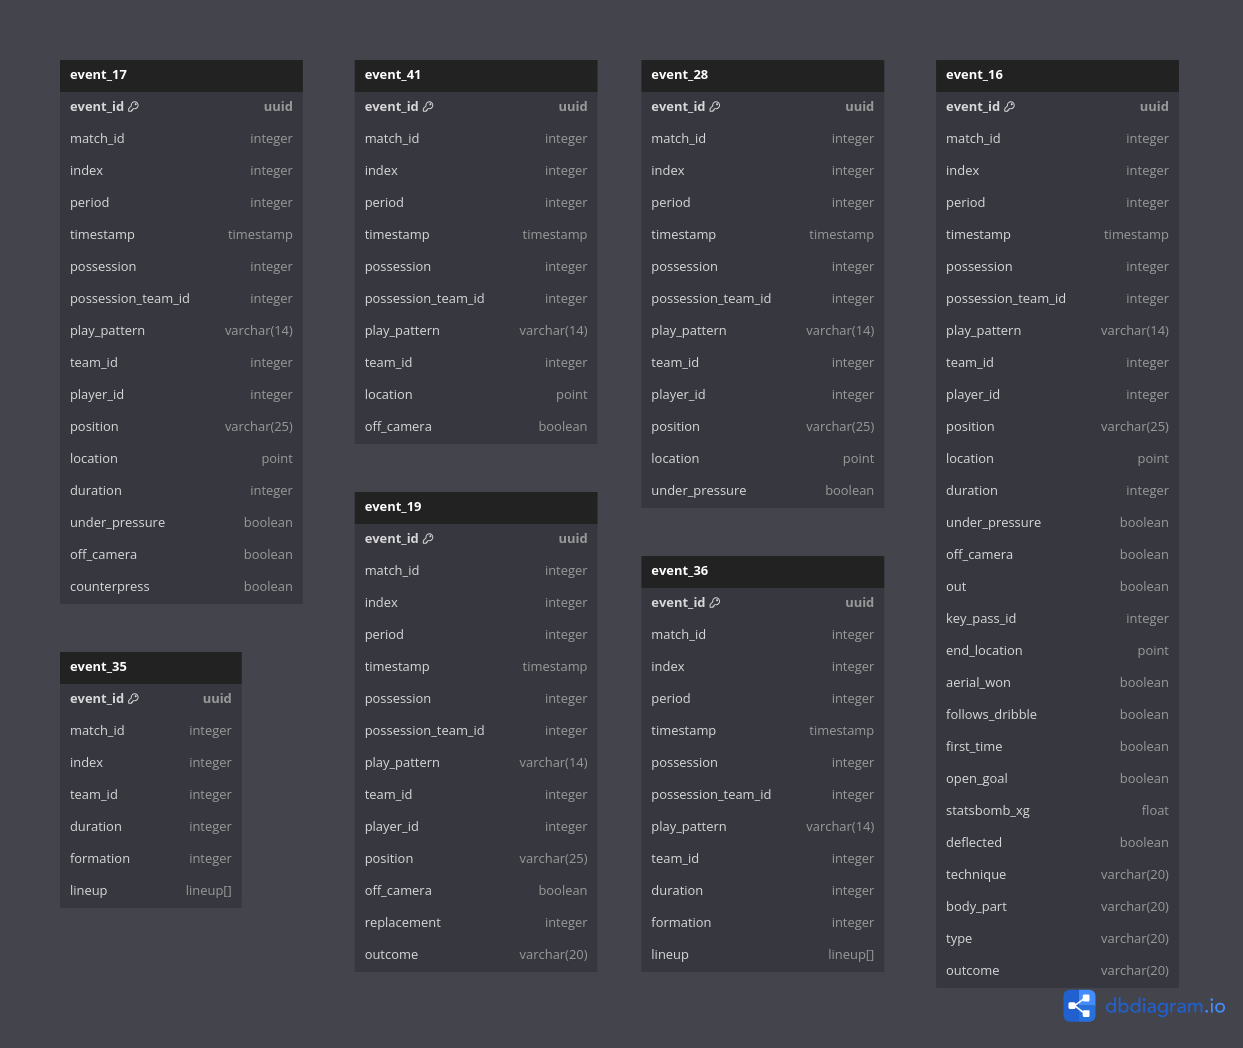
\includegraphics[width=\textwidth]{reduction/6.png}

\section*{Database Schema Diagrams}

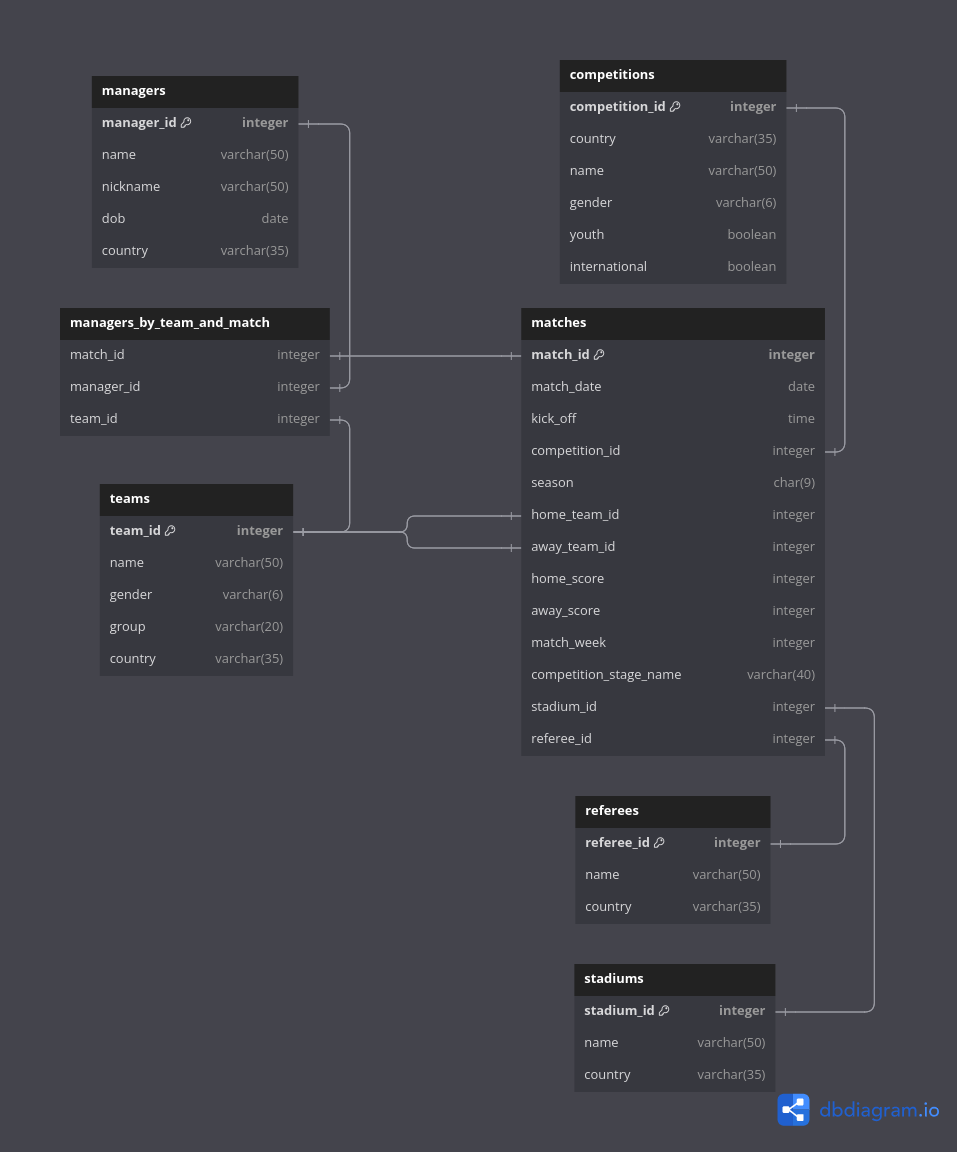
\includegraphics[width=\textwidth]{schema-diagram/matches_schema.png}
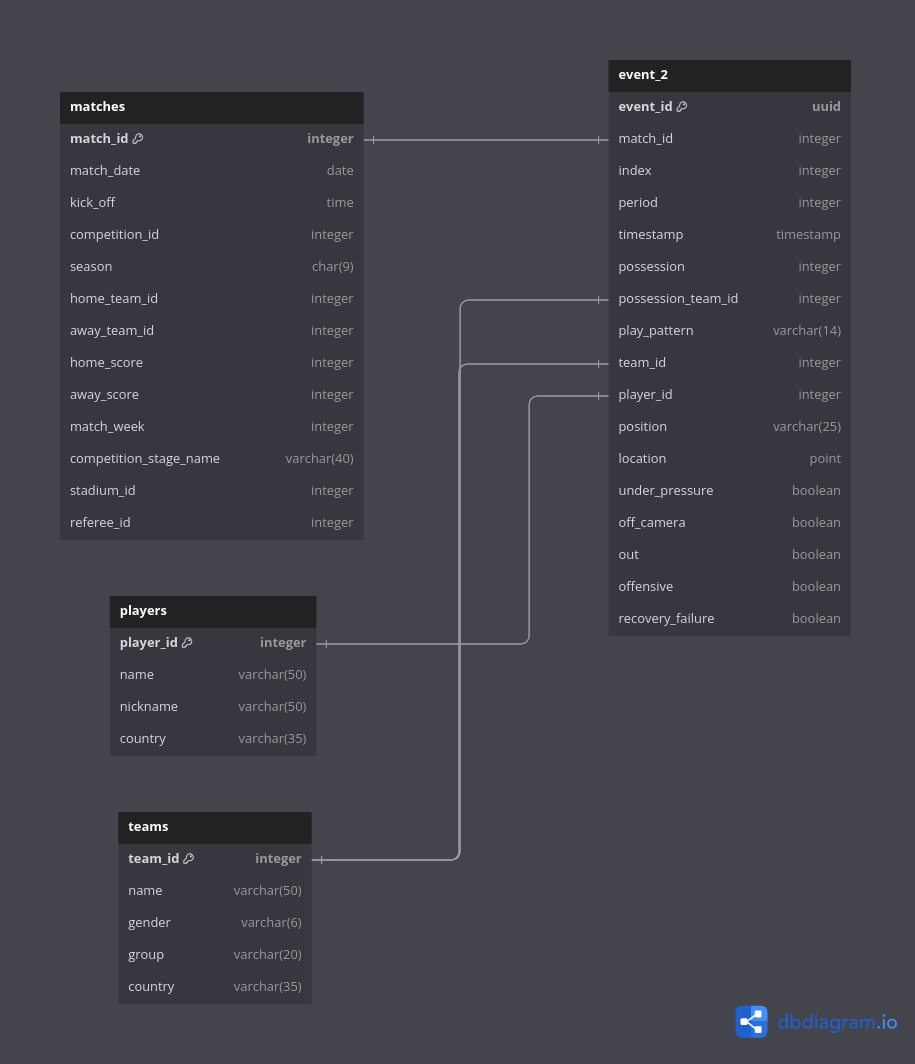
\includegraphics[width=\textwidth]{schema-diagram/event_2.png}
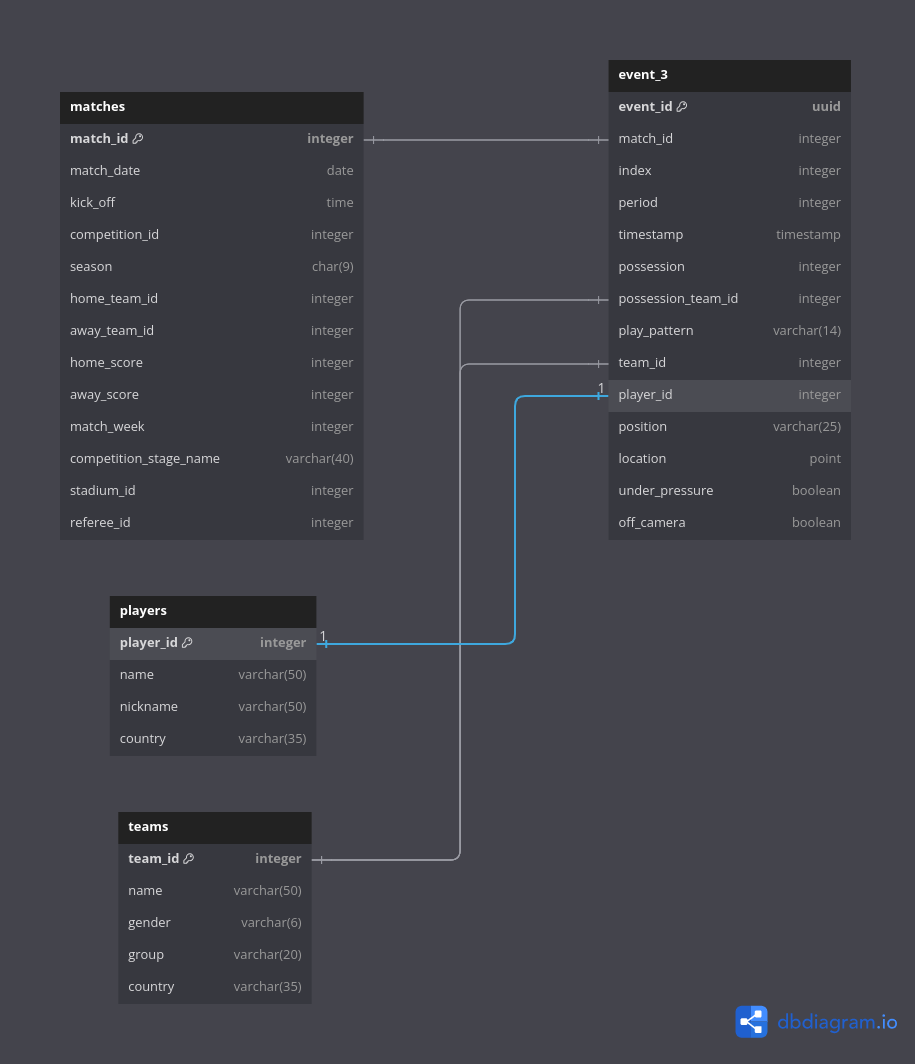
\includegraphics[width=\textwidth]{schema-diagram/event_3.png}
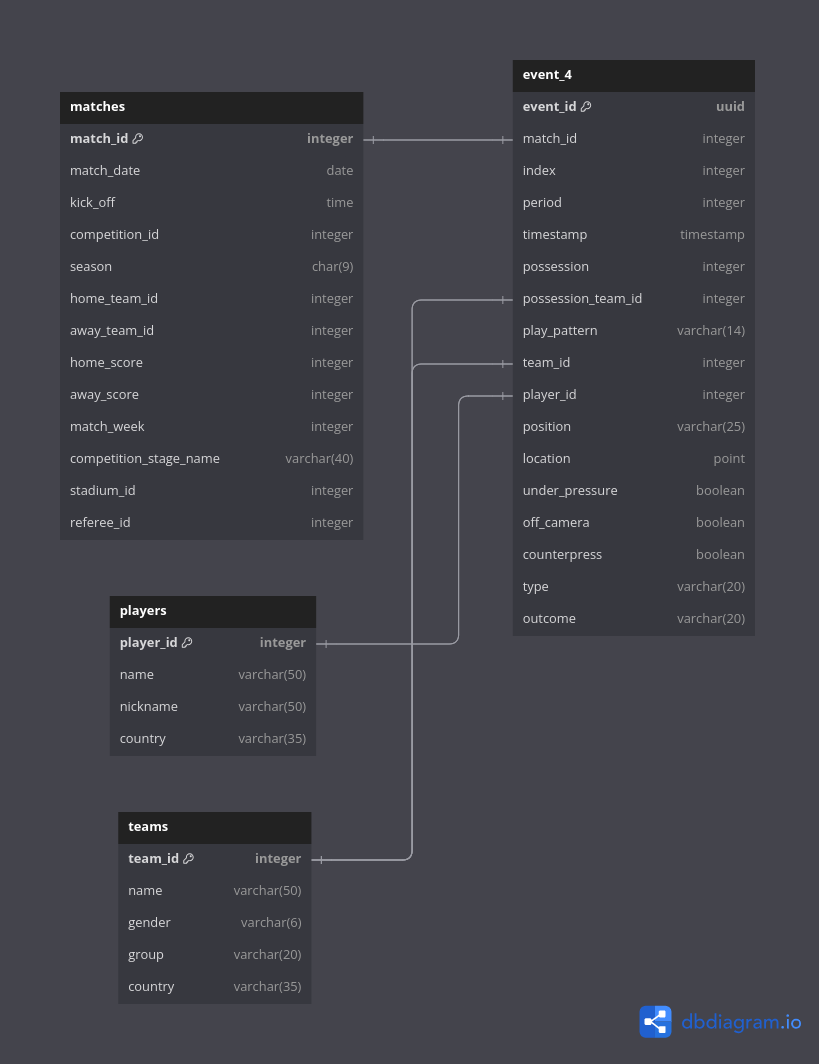
\includegraphics[width=\textwidth]{schema-diagram/event_4.png}
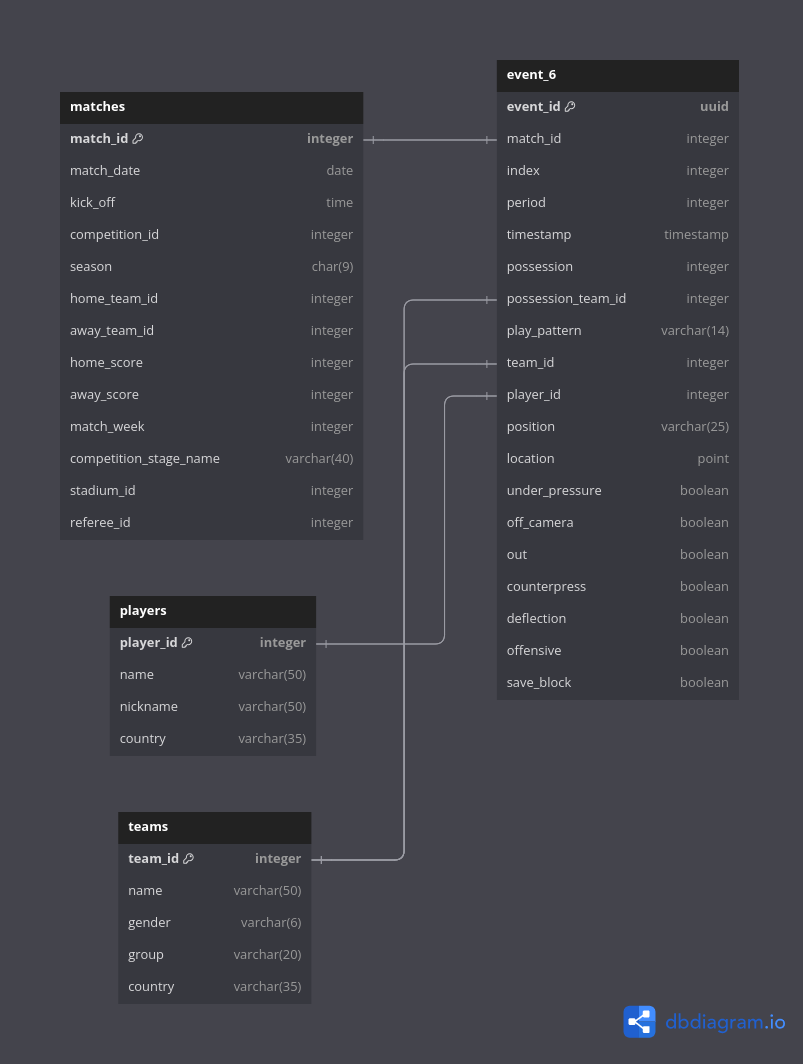
\includegraphics[width=\textwidth]{schema-diagram/event_6.png}
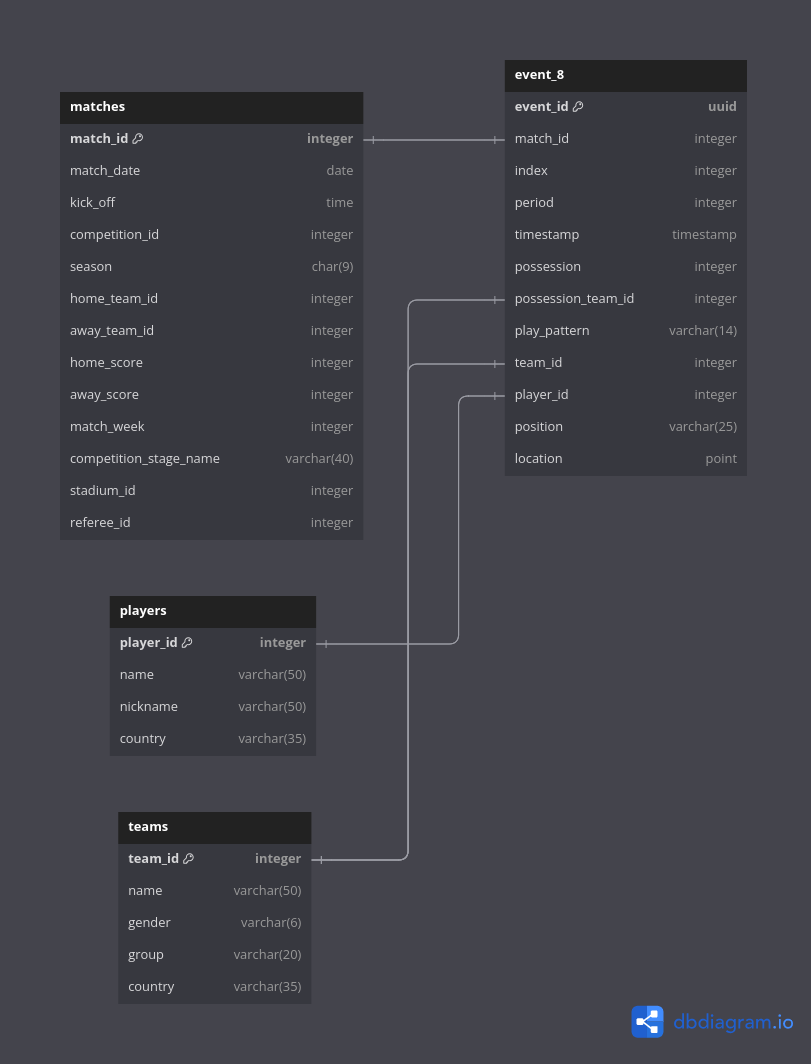
\includegraphics[width=\textwidth]{schema-diagram/event_8.png}
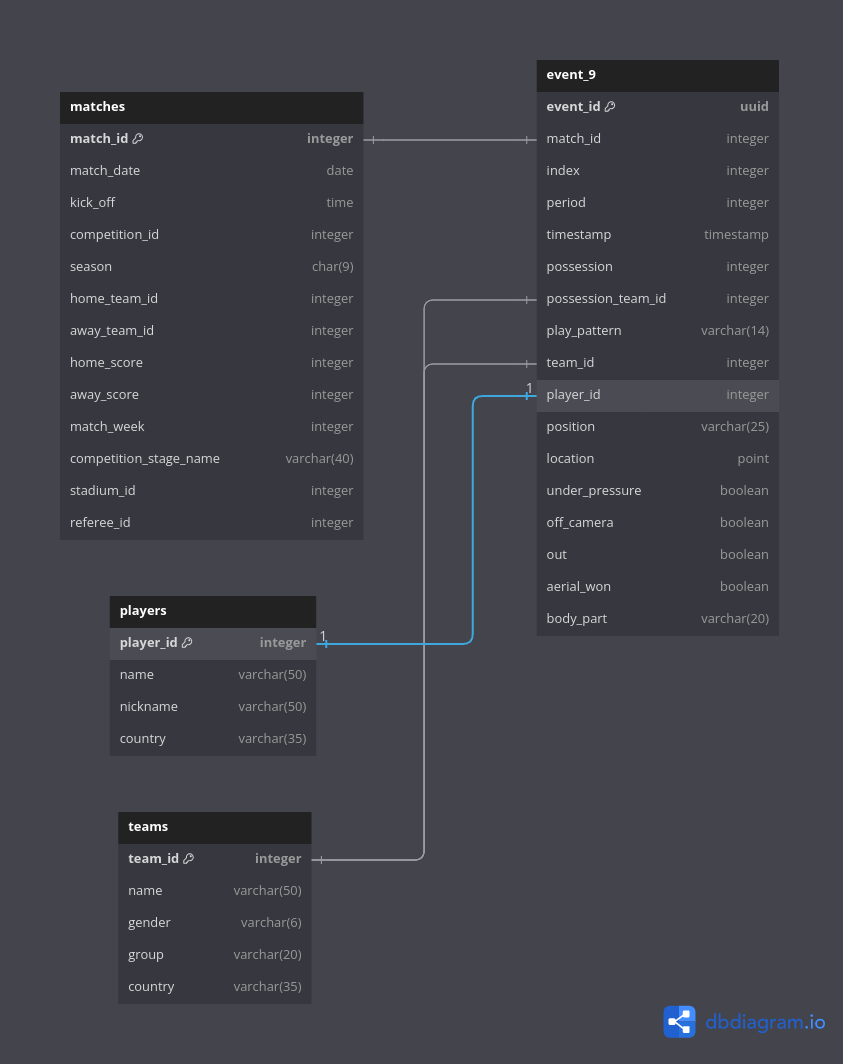
\includegraphics[width=\textwidth]{schema-diagram/event_9.png}
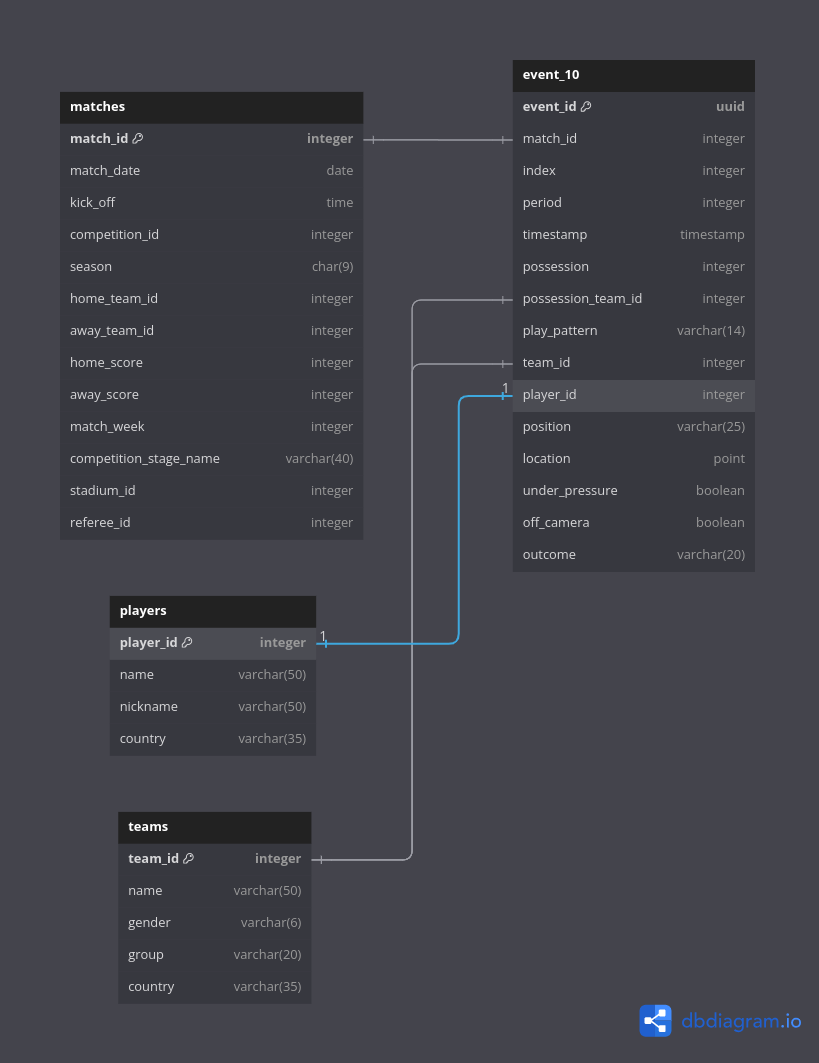
\includegraphics[width=\textwidth]{schema-diagram/event_10.png}
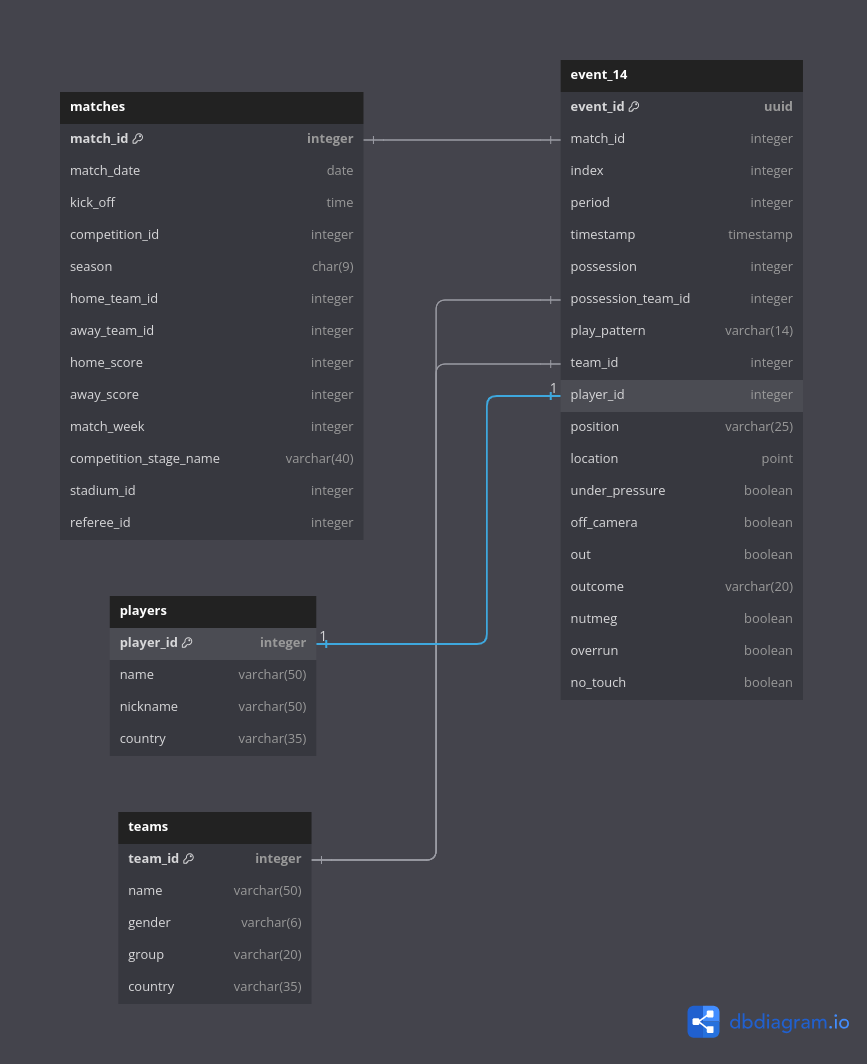
\includegraphics[width=\textwidth]{schema-diagram/event_14.png}
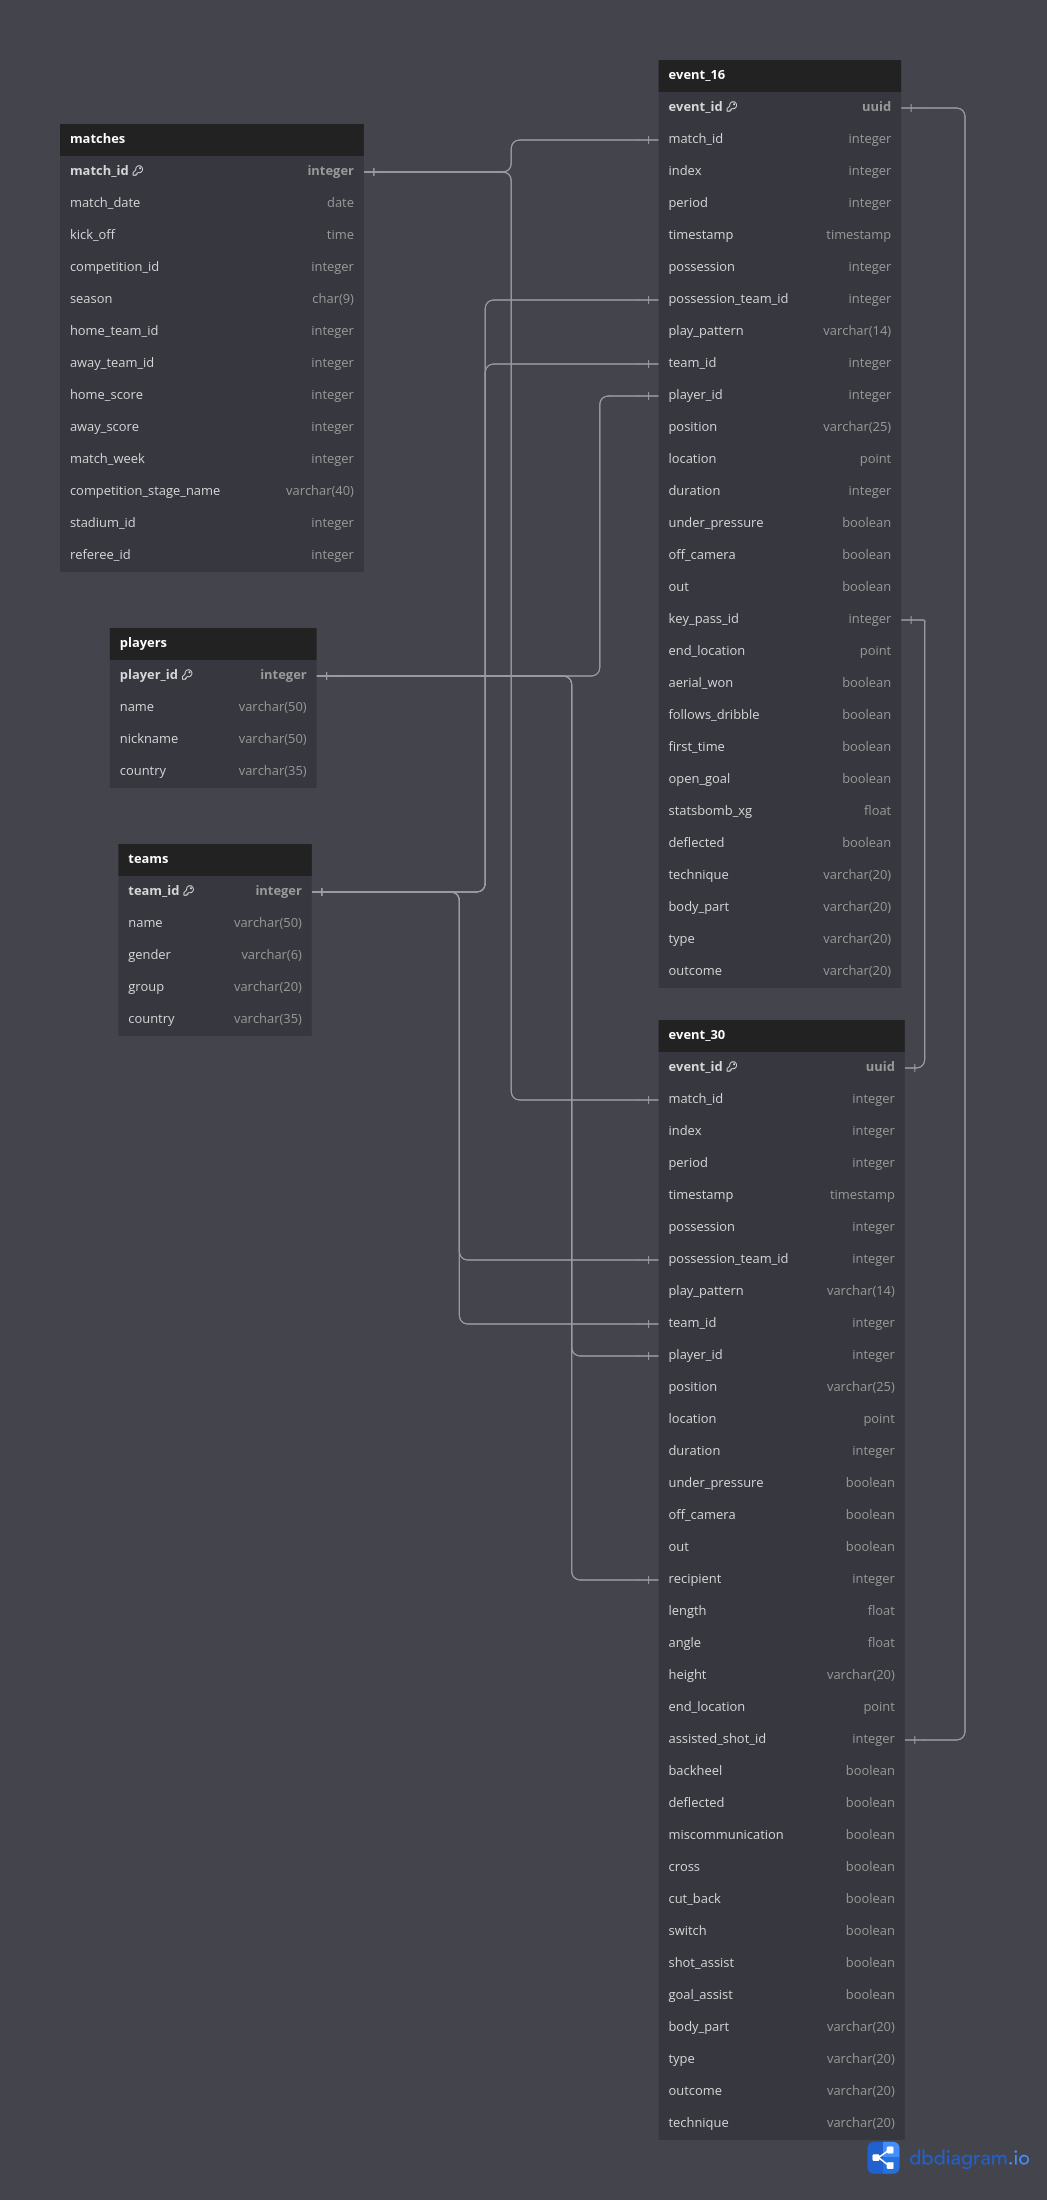
\includegraphics[width=\textwidth]{schema-diagram/event_16_30.png}
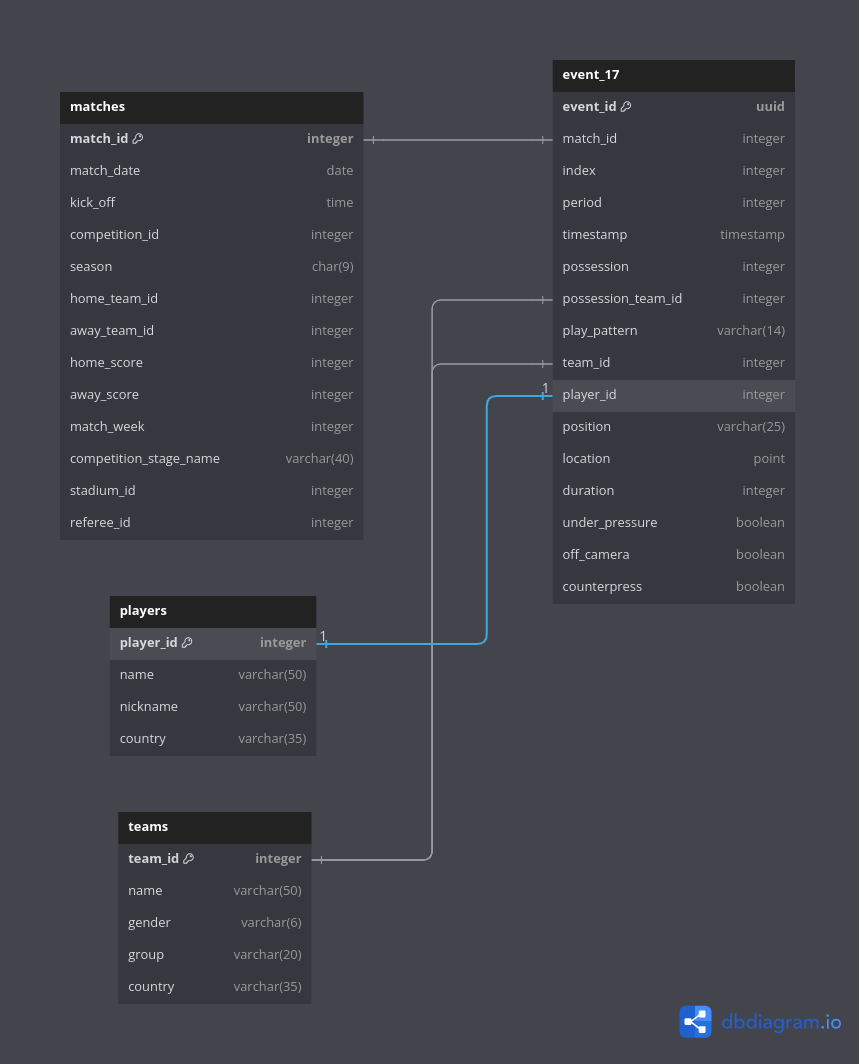
\includegraphics[width=\textwidth]{schema-diagram/event_17.png}
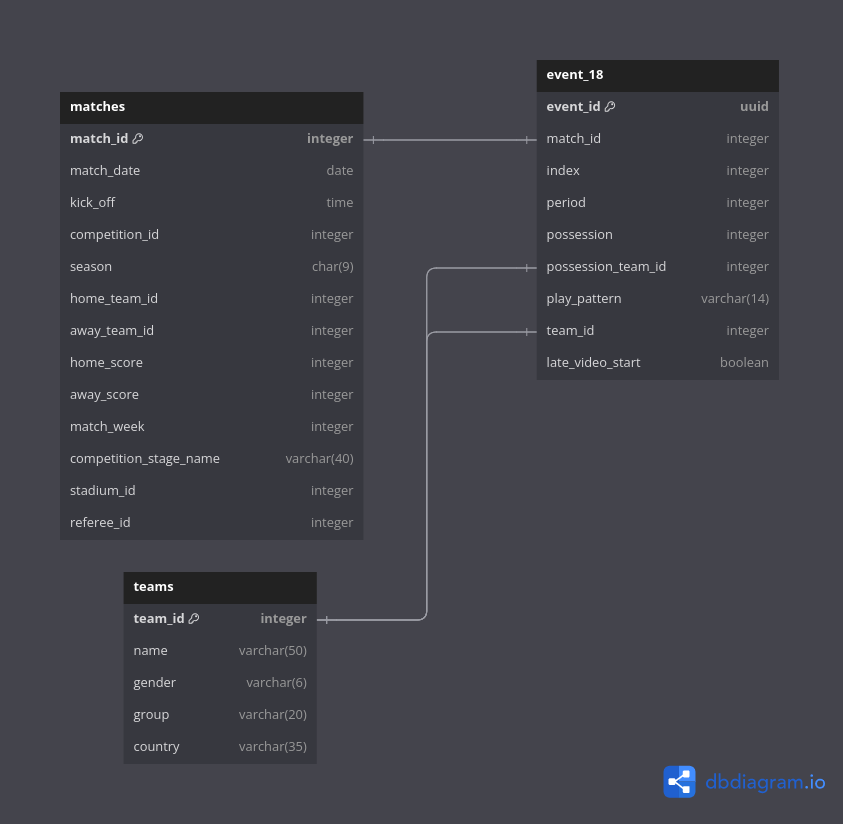
\includegraphics[width=\textwidth]{schema-diagram/event_18.png}
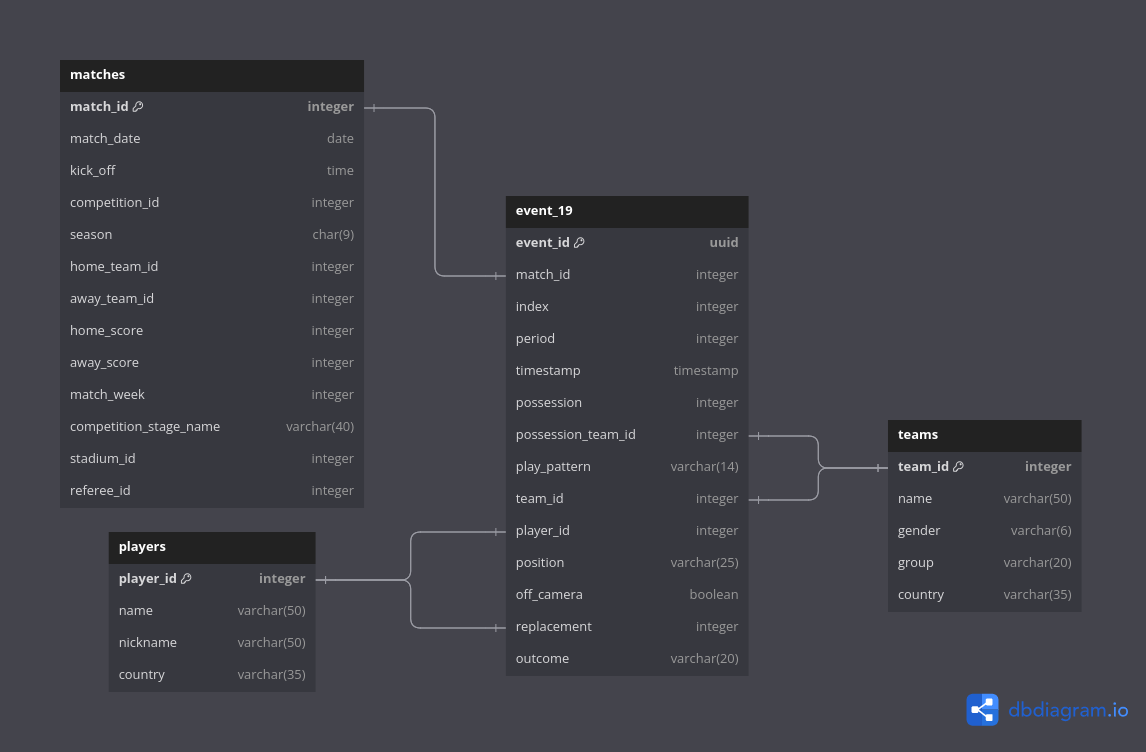
\includegraphics[width=\textwidth]{schema-diagram/event_19.png}
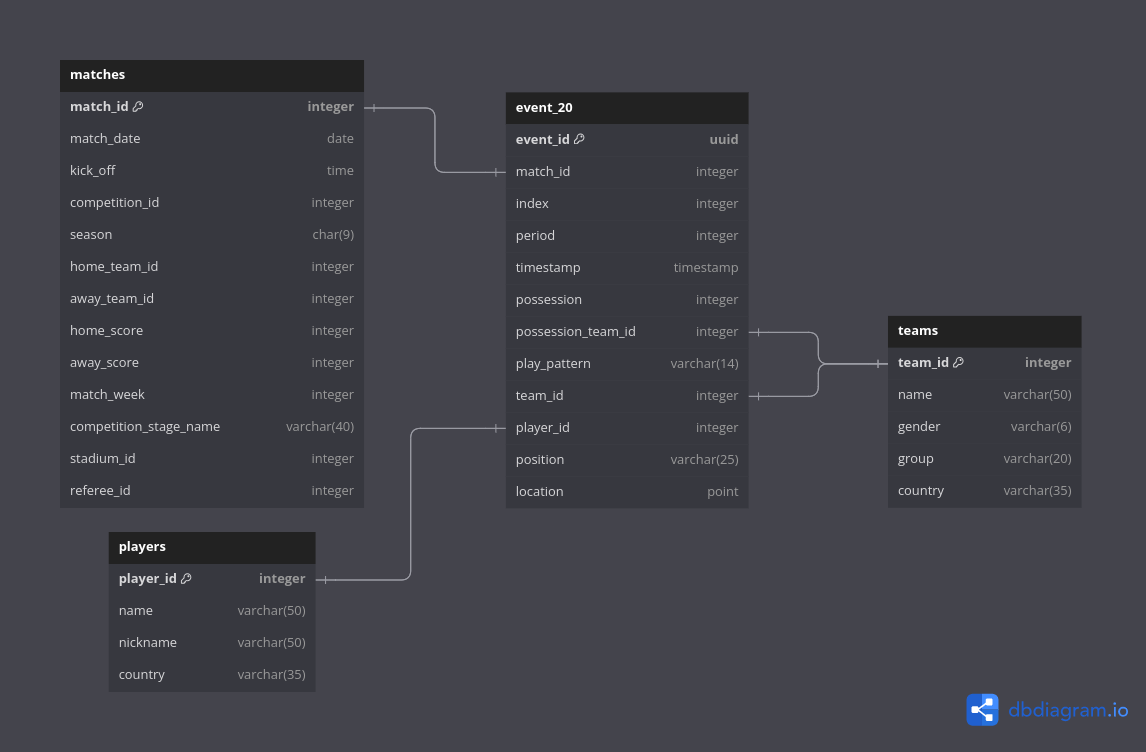
\includegraphics[width=\textwidth]{schema-diagram/event_20.png}
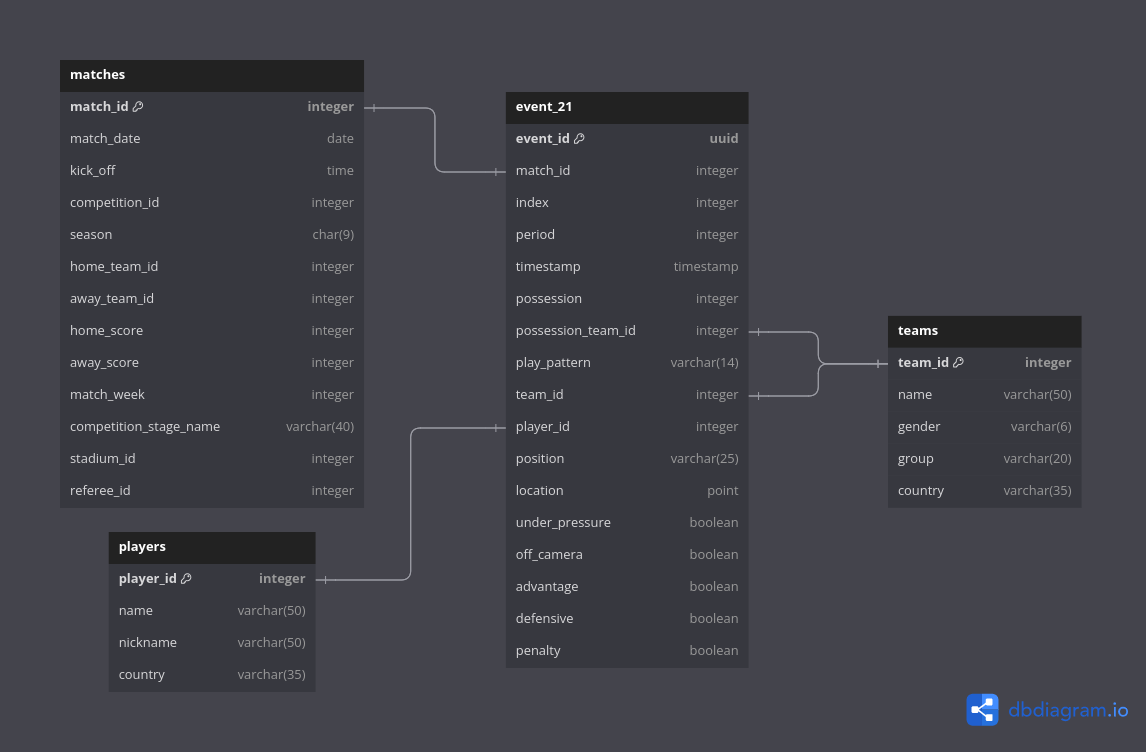
\includegraphics[width=\textwidth]{schema-diagram/event_21.png}
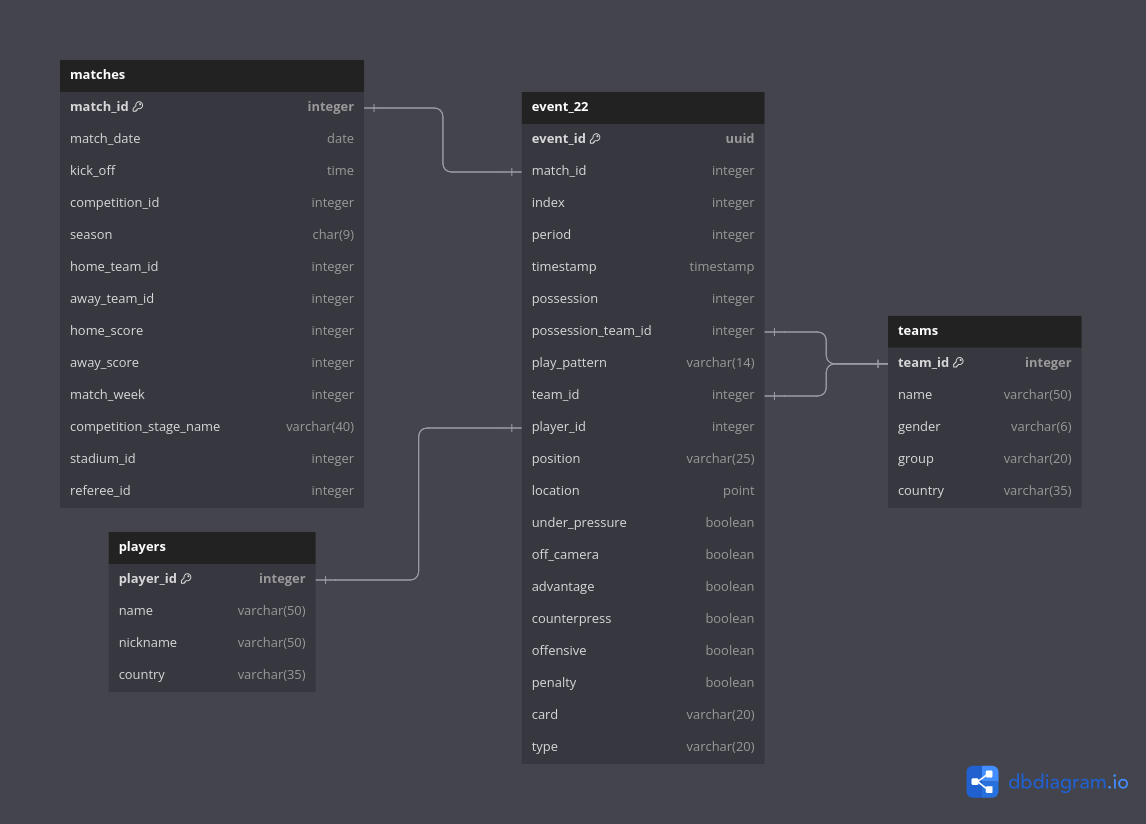
\includegraphics[width=\textwidth]{schema-diagram/event_22.png}
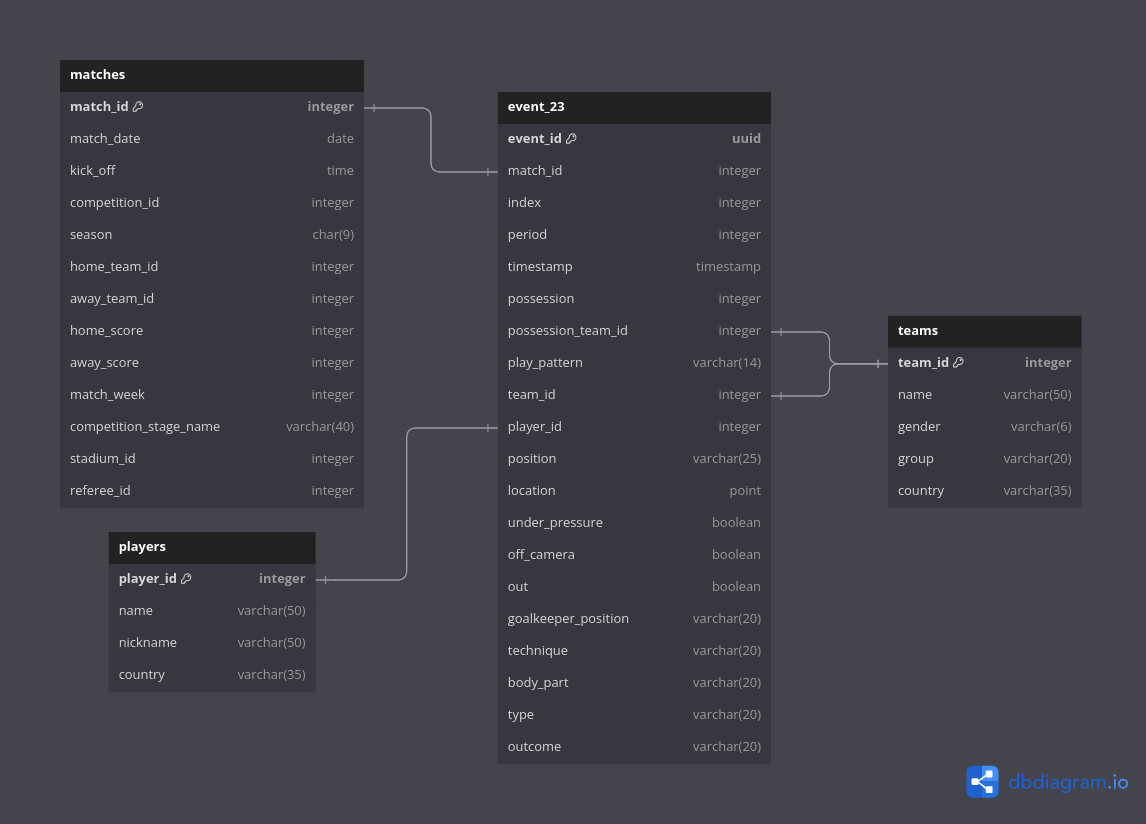
\includegraphics[width=\textwidth]{schema-diagram/event_23.png}
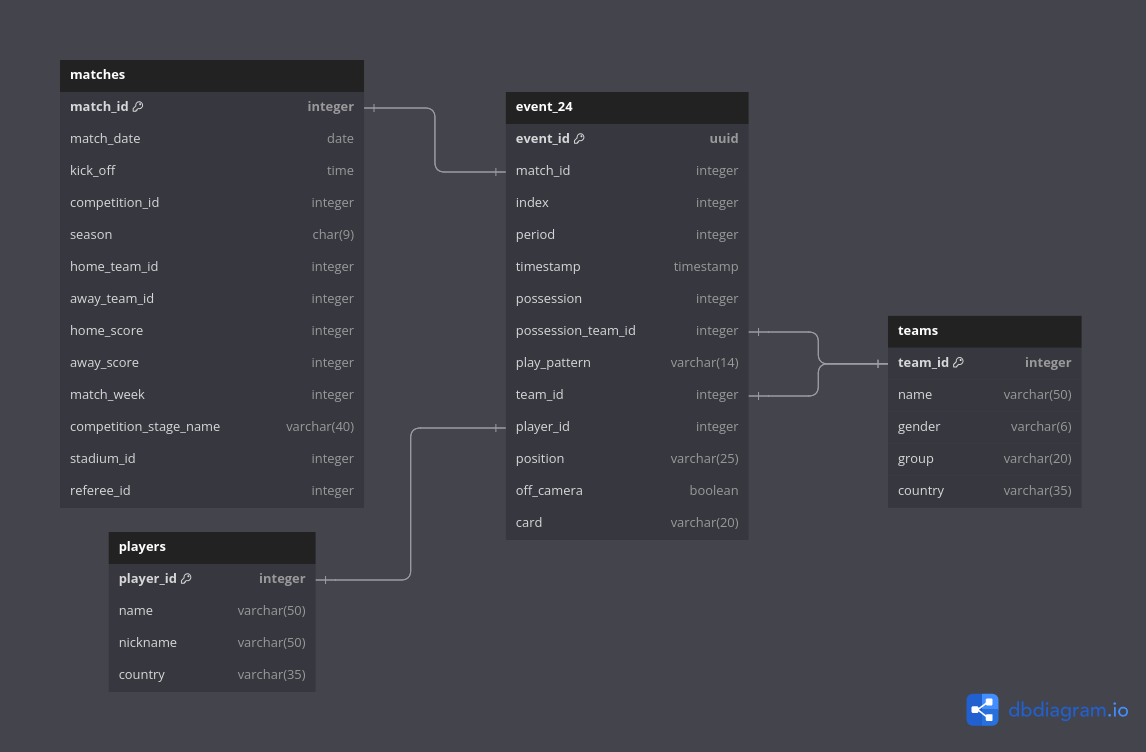
\includegraphics[width=\textwidth]{schema-diagram/event_24.png}
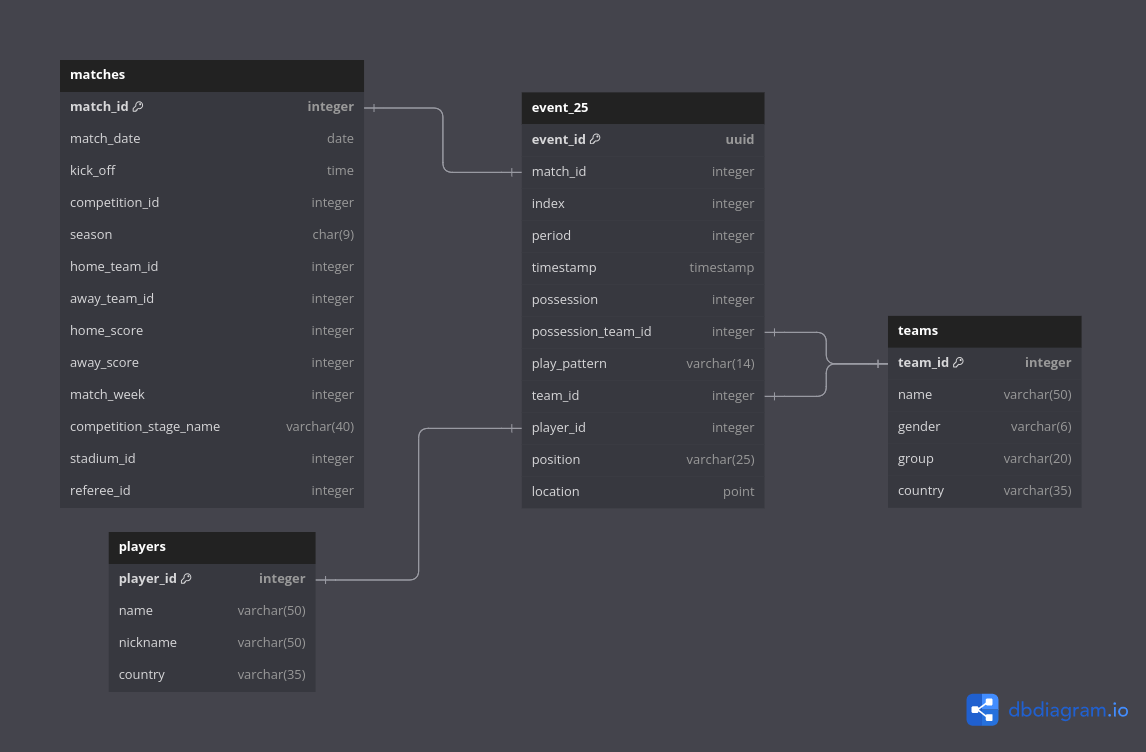
\includegraphics[width=\textwidth]{schema-diagram/event_25.png}
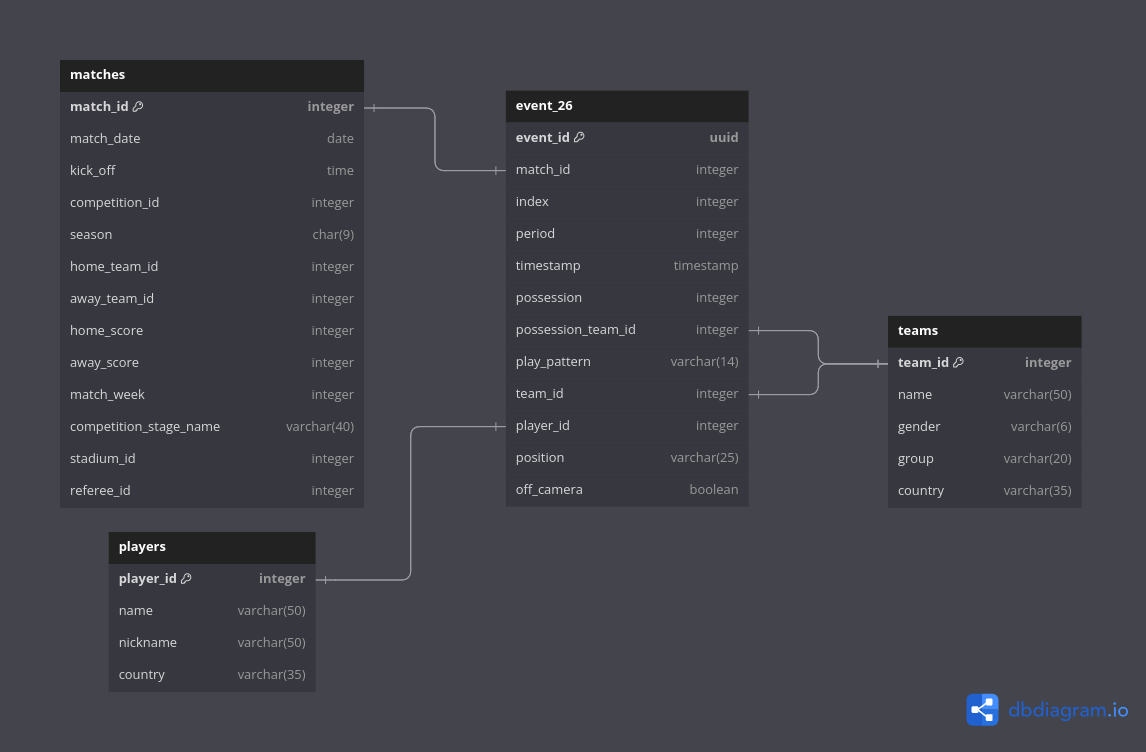
\includegraphics[width=\textwidth]{schema-diagram/event_26.png}
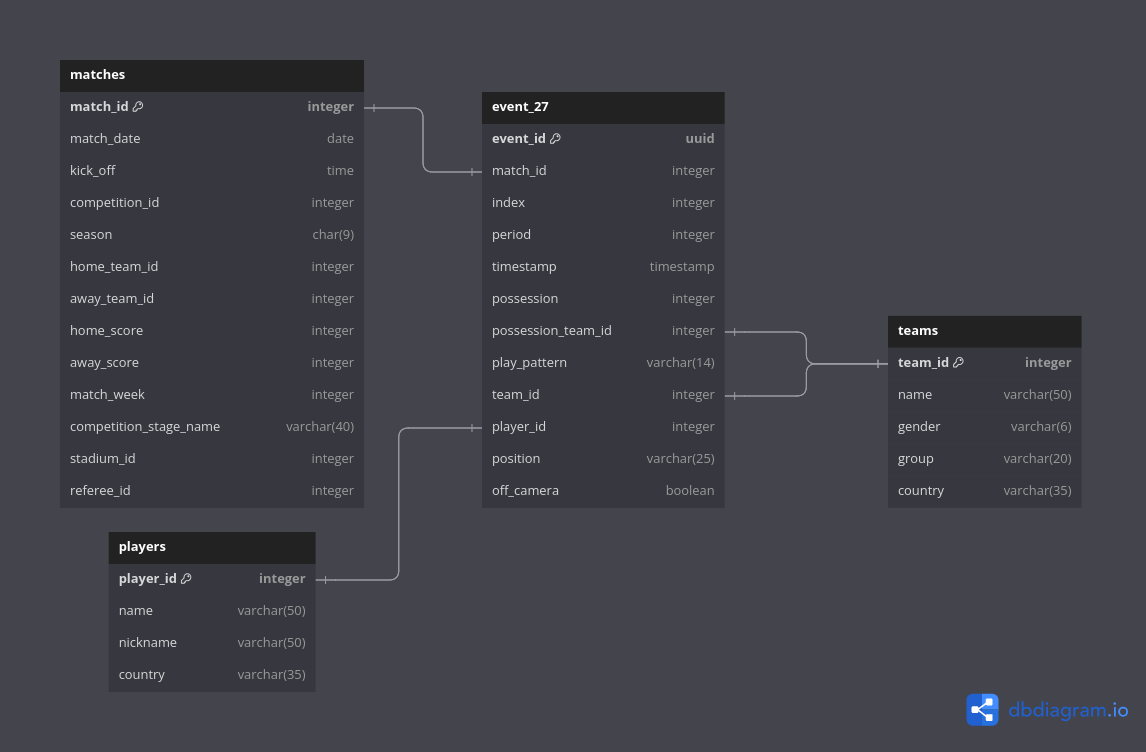
\includegraphics[width=\textwidth]{schema-diagram/event_27.png}
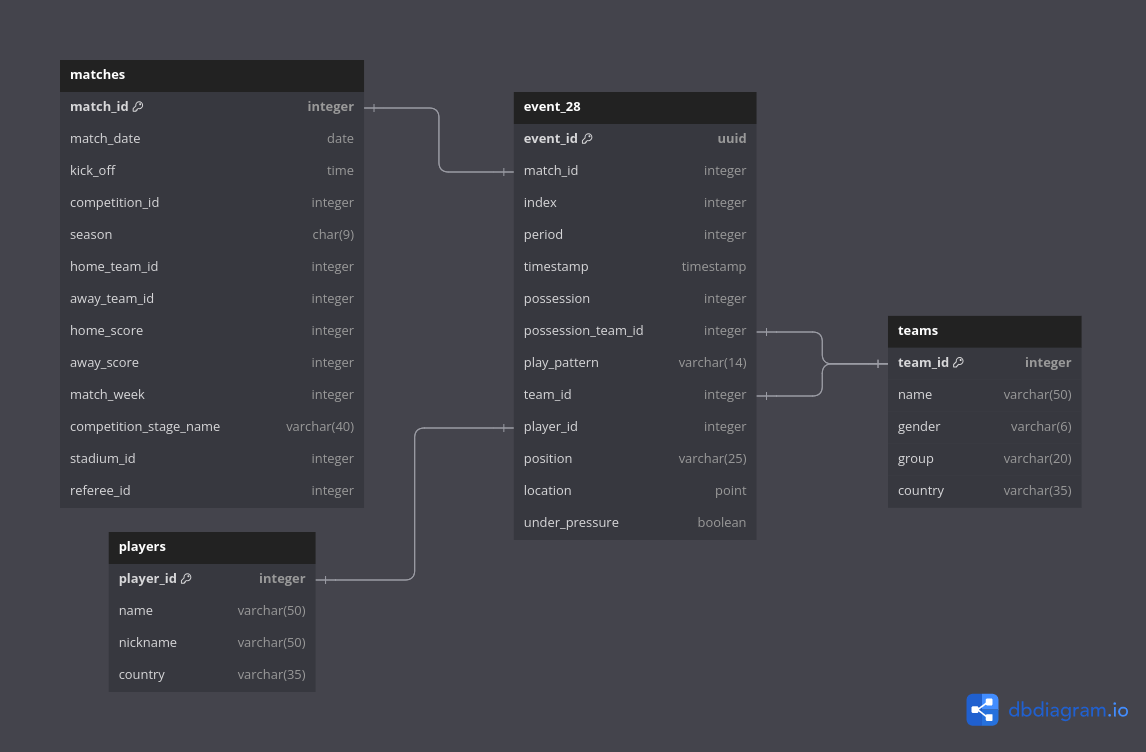
\includegraphics[width=\textwidth]{schema-diagram/event_28.png}
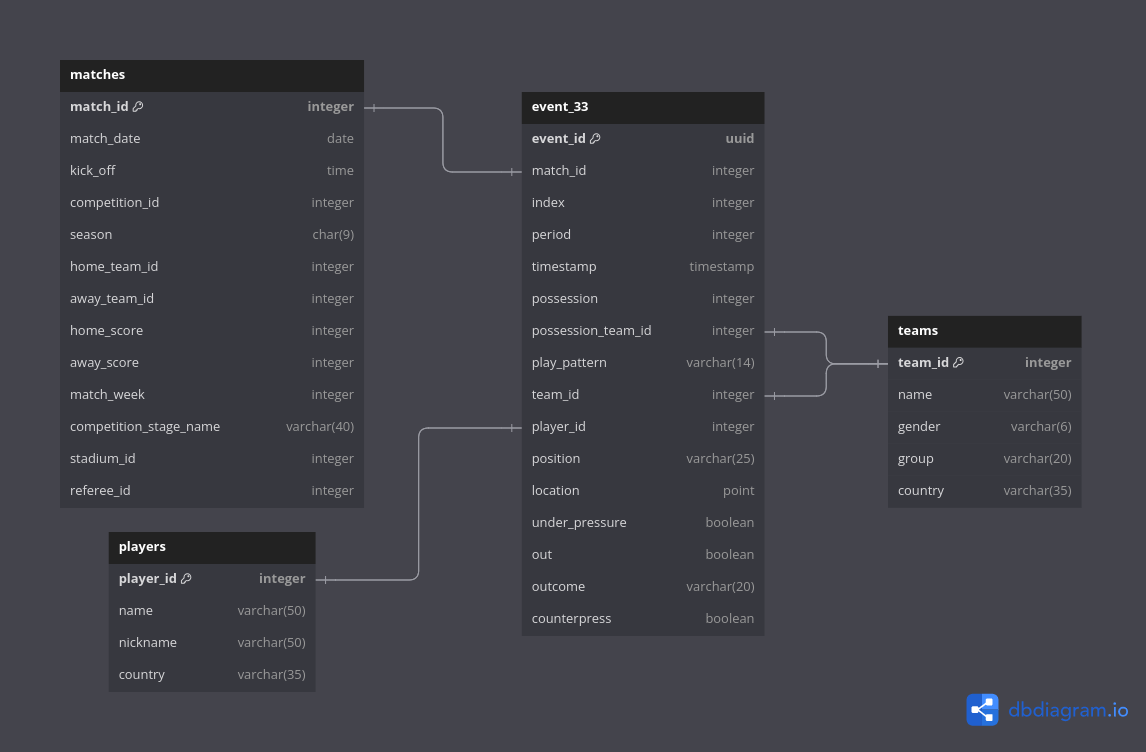
\includegraphics[width=\textwidth]{schema-diagram/event_33.png}
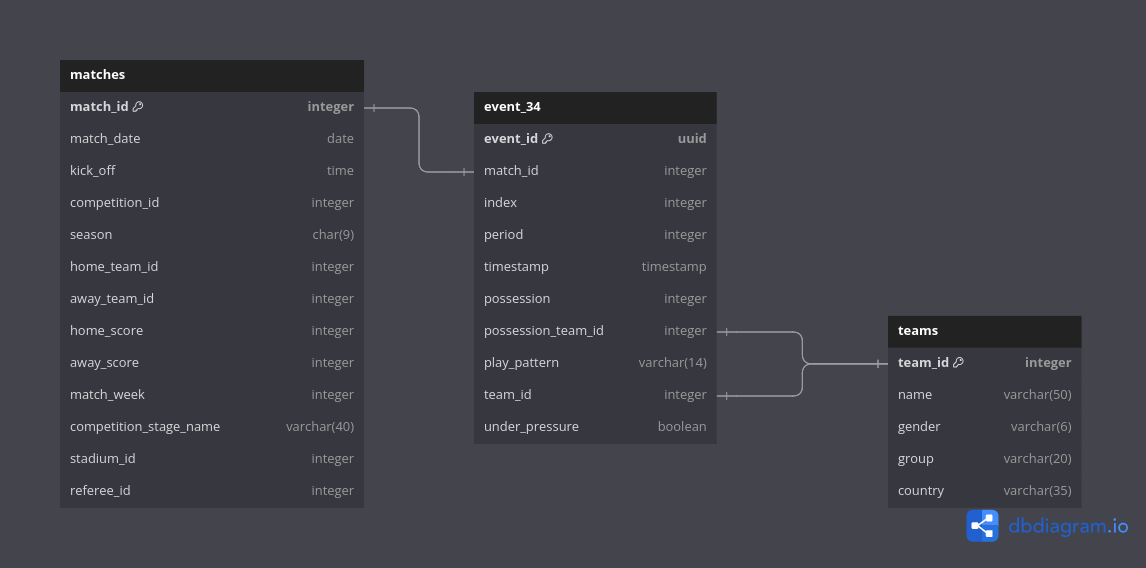
\includegraphics[width=\textwidth]{schema-diagram/event_34.png}
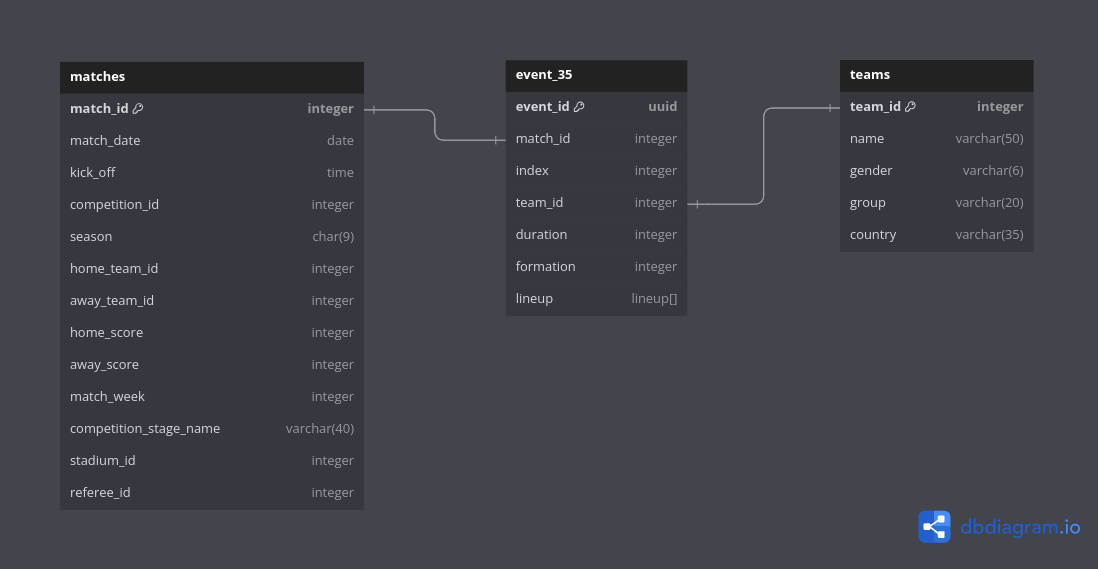
\includegraphics[width=\textwidth]{schema-diagram/event_35.png}
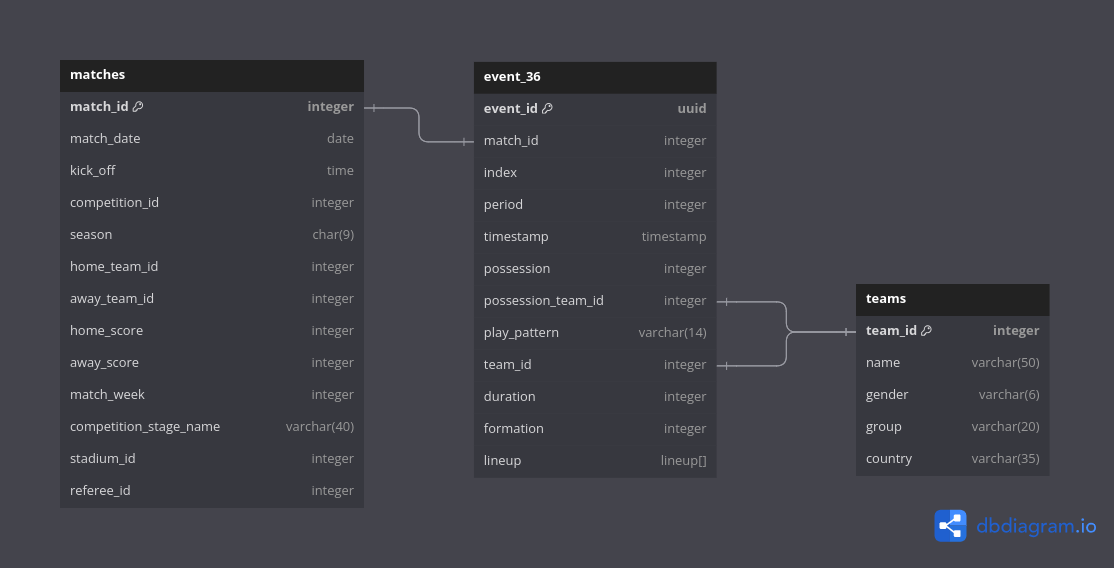
\includegraphics[width=\textwidth]{schema-diagram/event_36.png}
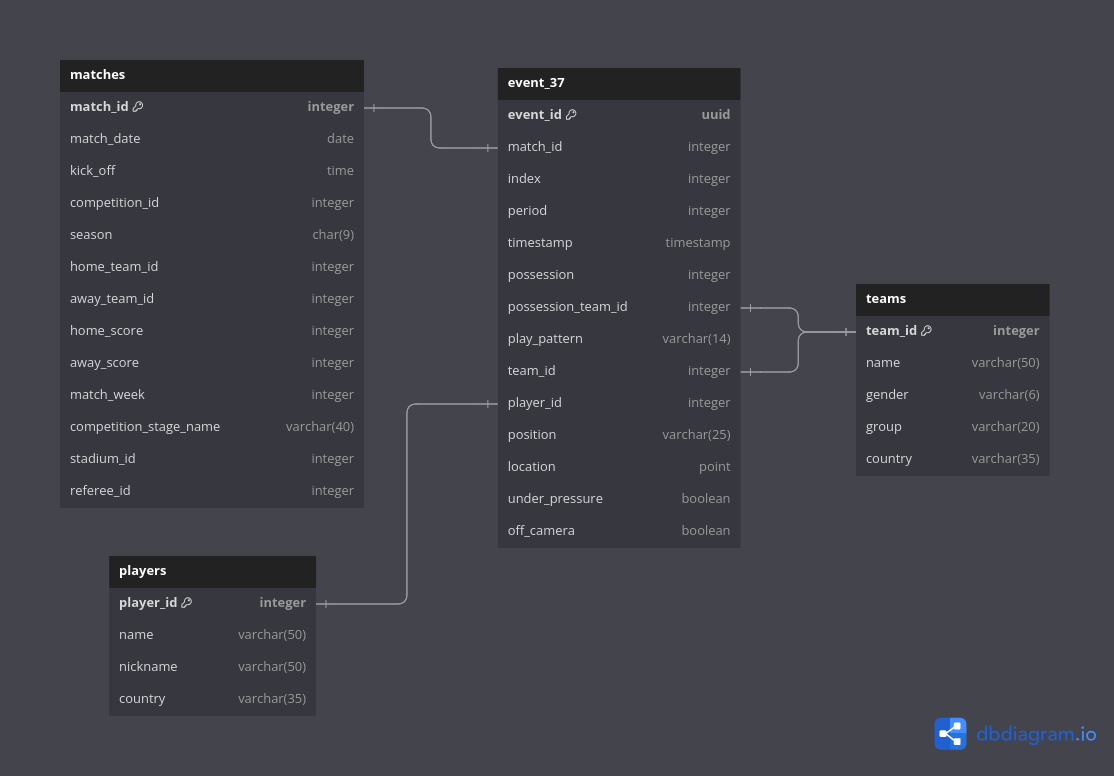
\includegraphics[width=\textwidth]{schema-diagram/event_37.png}
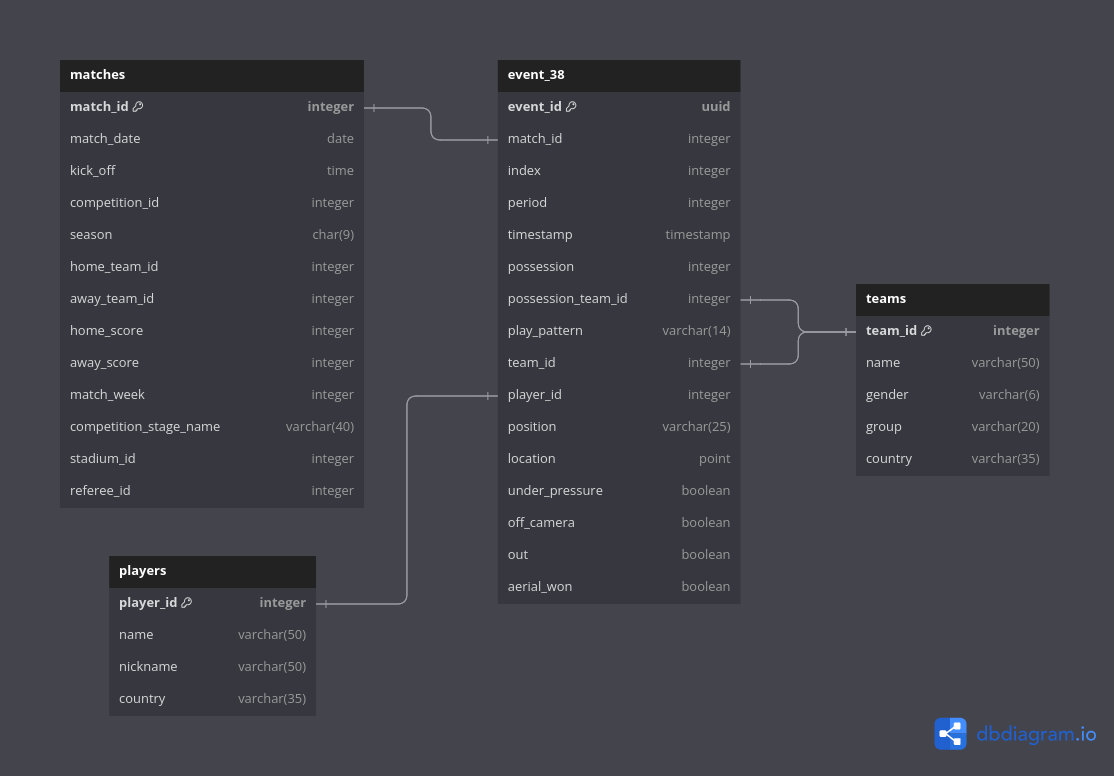
\includegraphics[width=\textwidth]{schema-diagram/event_38.png}
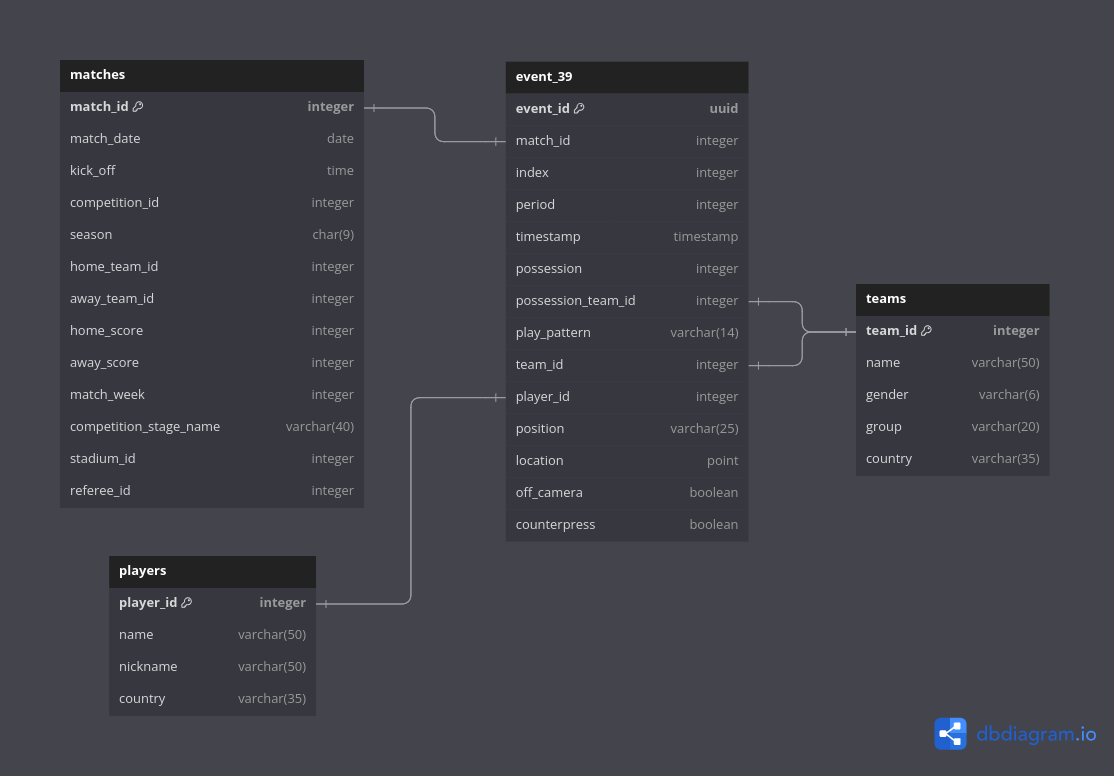
\includegraphics[width=\textwidth]{schema-diagram/event_39.png}
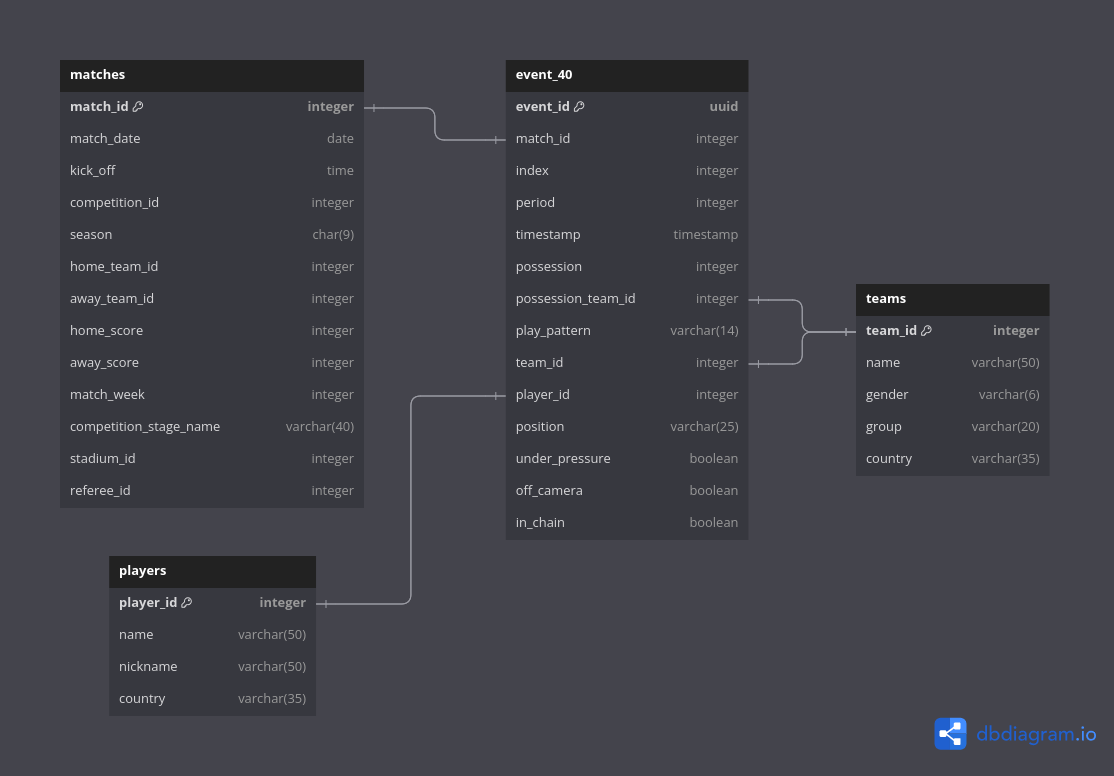
\includegraphics[width=\textwidth]{schema-diagram/event_40.png}
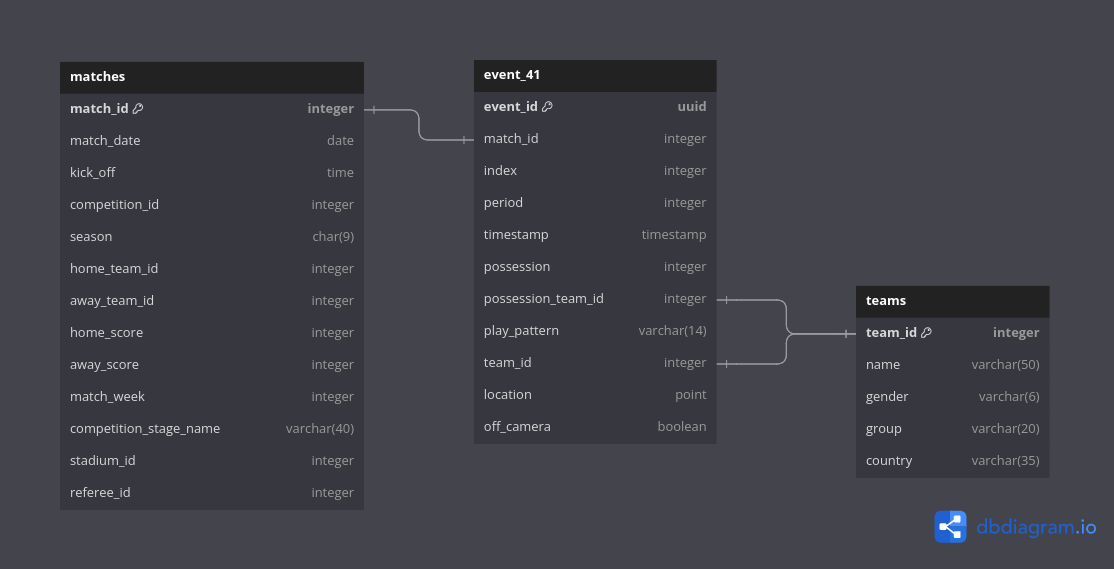
\includegraphics[width=\textwidth]{schema-diagram/event_41.png}
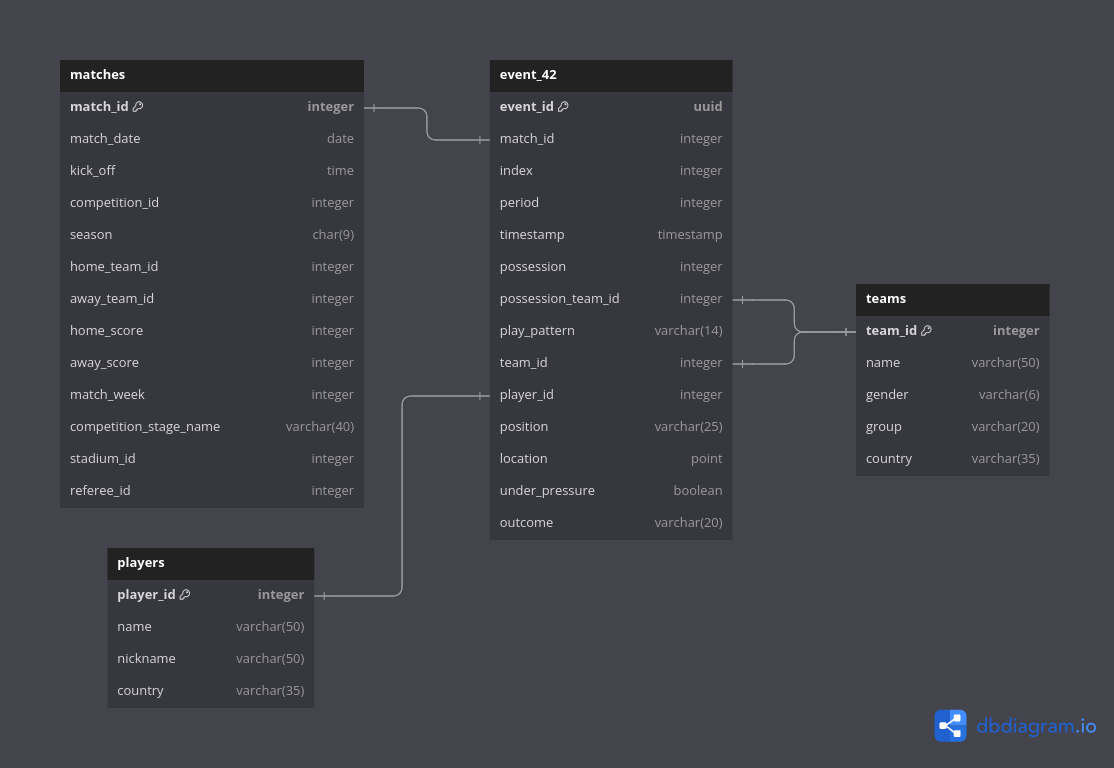
\includegraphics[width=\textwidth]{schema-diagram/event_42.png}
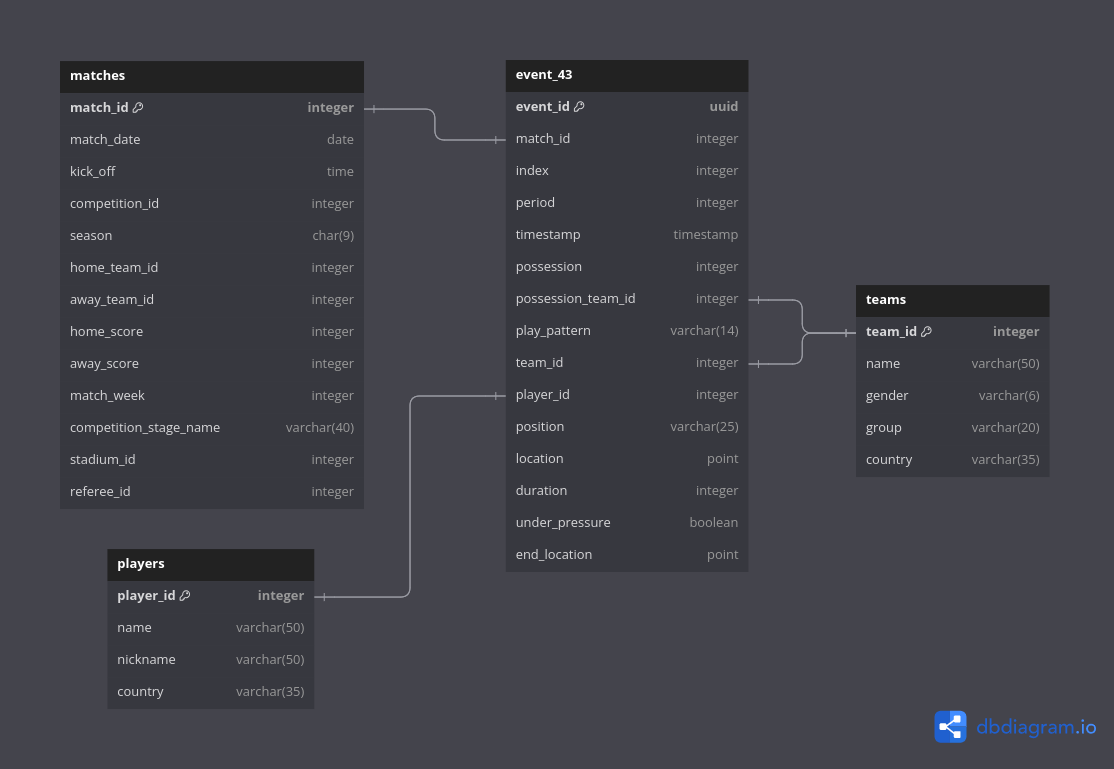
\includegraphics[width=\textwidth]{schema-diagram/event_43.png}

\end{document}
